\documentclass[10pt]{beamer}


\usepackage{lmodern} 		% Diese beiden packages sorgen für echte 
\usepackage[T1]{fontenc}	% Umlaute.

\usepackage{amssymb, amsmath, color, graphicx, float, setspace, tipa}
\usepackage[utf8]{inputenc} 
\usepackage[english]{babel}
\usepackage[justification=centering]{caption}
\addto\captionsenglish{\renewcommand{\figurename}{}} %Abbildungen nicht bzw. anders beschriften.


%\usepackage[pdfpagelabels,pdfstartview = FitH,bookmarksopen = true,bookmarksnumbered = true,linkcolor = black,plainpages = false,hypertexnames = false,citecolor = black, breaklinks]{hyperref}
%\usepackage{url}
%\usepackage{picins} 		%Gleittext um Grafik. Befehl: parpic. Vorlage siehe unten
\usepackage{longtable} 		%Seitenübergreifende Tabelle. Vorlage siehe unten
\newtheorem*{bem}{Bemerkung} % Neue Theorem-Umgebung: Bemerkung
\newcommand{\fillframe}{\vskip0pt plus 1filll} 
\newcommand{\musr}{$\mu$SR }

\usepackage{units}
\newcommand{\half}{\nicefrac{1}{2}}

\usepackage{tikz}
\usetikzlibrary{patterns}

\usepackage{grffile} %allow image filenames.that.include.dots.png



%-----------------
%BEAMER-SPEZIFISCH
%-----------------


\usetheme{metropolis}
%deactivate a new page when a new section begins
\metroset{sectionpage=none} 
\usepackage{FiraSans}
\usefonttheme[onlymath]{serif}



% Verschiedene Varianten von usetheme, usecolortheme und usefonttheme kann man hier ausprobieren: http://deic.uab.es/~iblanes/beamer_gallery/


%Halbtransparente Overlays (was als nächstes Element auf der Folie gezeigt wird)
%\setbeamercovered{transparent} 

% Entfernt Navigationssymbole unten
%\beamertemplatenavigationsymbolsempty 

% Seitenzahlen als links
%\setbeamertemplate{footline}[frame]  
%    \setbeamertemplate{footline}{%
%    	\raisebox{5pt}{\makebox[\paperwidth]{\hfill\makebox[10pt]{\hyperlink{tableofcontents}{\scriptsize\insertframenumber}}}}}






%---------------------
%--Metainformationen--
%---------------------
\title{Advection Project}


\author[M. Ivkovic]{Mladen Ivkovic}
\date{January 2018}



% \title[Kurzform]{Vortrag zur Berechenbarkeit}
%     Titel des Vortrages
% \subtitle[Kurzform]{Untertitel}
%     Untertitel
% \author[M. Schulz]{Michael Schulz}
%     Autor festlegen
% \institute[IfI -- HU Berlin]{Institut für Informatik\\ Humboldt-Universität zu Berlin}
%     Angabe des Institutes
% \date[26.05.06]{26. Mai 2006}
%     Datum der Präsentation, alternativ kann mittels \date{\today} auch das aktuelle Datum eingetragen werden.
% \logo{\pgfimage[width=2cm,height=2cm]{hulogo}}
%     Die Datei hulogo.pdf (bzw. hulogo.png, hulogo.jpg, hulogo.mps bei Verwendung von pdftex als Backend) als Logo auf allen Folien, hier mithilfe des Paketes pgf.
% \titlegraphic{\includegraphics[width=2cm,height=2cm]{hulogo}}
%     Die Datei hulogo.pdf (bzw. analog wie bei \logo auch entsprechendes Format) als Logo nur auf der Titelseite unter Verwendung des Paketes graphicx.








%===================================================================================
%===================================================================================
% \begin{frame}[Overlay-Aktionen][Optionen]{Titel}{Untertitel}
% 
% Overlay-Aktionen
%     Overlay-Aktionen setzen die Standard-Overlay-Aktionen aller Umgebungen innerhalb des Frames, welche Aktion-Spezifikationen erlauben. Dazu gehören u.a. \item bei Listen und Block-Umgebungen.
% 
%     <+->
%         Sorgt dafür, dass die Elemente stückweise zum Vorschein kommen.
% 
% Optionen
% 
%     allowdisplaybreaks
%         Sorgt durch Aufruf von \allowdisplaybreaks aus AMS-LaTeX für einen Seitenumbruch bei mehrzeiligen Formelumgebungen. Funktioniert nur im Zusammenhang mit der Option allowframebreaks
%     allowframebreaks
%         Passt der Inhalt nicht mehr auf ein Slide, wird er automatisch auf mehrere Slides verteilt. Allerdings ist somit kein Overlay mehr möglich.
%     b,c,t
%         Sorgt dafür, dass der Frame nach unten (b), zentriert (c) oder nach oben (t) ausgerichtet wird.
%     fragile
%         Wird für Quelltextumgebungen, z.B. verbatim, benötigt.
%     label=name
%         Legt einen Namen für ein Frame fest um es später mit \againframe{name} erneut aufrufen zu können.
%     plain
%         Unterdrückt die Anzeige der Überschrift, Fußzeile und Sidebar.
%     squeeze
%         Verkleinert die vertikalen Abstände so weit wie möglich um u.U. mehr auf der Folie unterbringen zu können.
% 
%===================================================================================
%===================================================================================




\begin{document}


\begin{frame}{}
	\titlepage
\end{frame}

%\section{Introduction}
%\begin{frame}
	\frametitle{Introduction}
	
	Goal: Calculation of gravitational force on a system of collisionless particles
	
	Possible methods:
	
	\begin{itemize}
		\item Direct calculation
		\item Iterative methods on a mesh
		\item Fourier methods on a mesh
		\item Tree methods (hierarchical multipole methods)
	\end{itemize}

	In this project, I implemented a direct calculation and a tree method.
\end{frame}







\begin{frame}
	\frametitle{Dataset}
	The dataset for which to compute the forces is a set of $\sim 50'000$ particles aranged according to the spherically symmetric ``Hernquist model'' :
	\begin{align*}
		\rho(r) &= \frac{M}{2\pi}\frac{a}{r}\frac{1}{(r+a)^3}\\
		M(r) &= M \frac{r^2}{(r+a)^2} \quad\quad \Rightarrow M(a) = \frac{M}{4}\\
		\phi(r) &= - \frac{GM}{r+a}
	\end{align*}
\end{frame}




\begin{frame}
	\frametitle{Choice of Units}
	
	Use dimensionless units, with $G \equiv 1$
	
	$\Rightarrow$ Reduce number of multiplications necessary
	
	$\Rightarrow$ Reduce effect of finite floating point precision by moving problem to a better suited order of magnitude
	
	Define a scale for every physical quantity:
	\begin{align*}
		a_{phys} \equiv A_0 a_{code}
	\end{align*}
	
	Setting $G = 1$ restricts the scale for either time, mass or distance. I chose
	\begin{align*}
		M_0 &= M_{tot}	\quad\quad &\text{ such that } \quad M_{tot, code} = 1\\
		R_0 &= R_{max}	\quad\quad &\text{ such that } \quad R_{max, code} = 1\\
		\Rightarrow \quad T_0 &= \sqrt{ \frac{R_0^3}{G M_0}} &
	\end{align*}
	
\end{frame}





\begin{frame}
	\frametitle{Dataset}
	\centering
	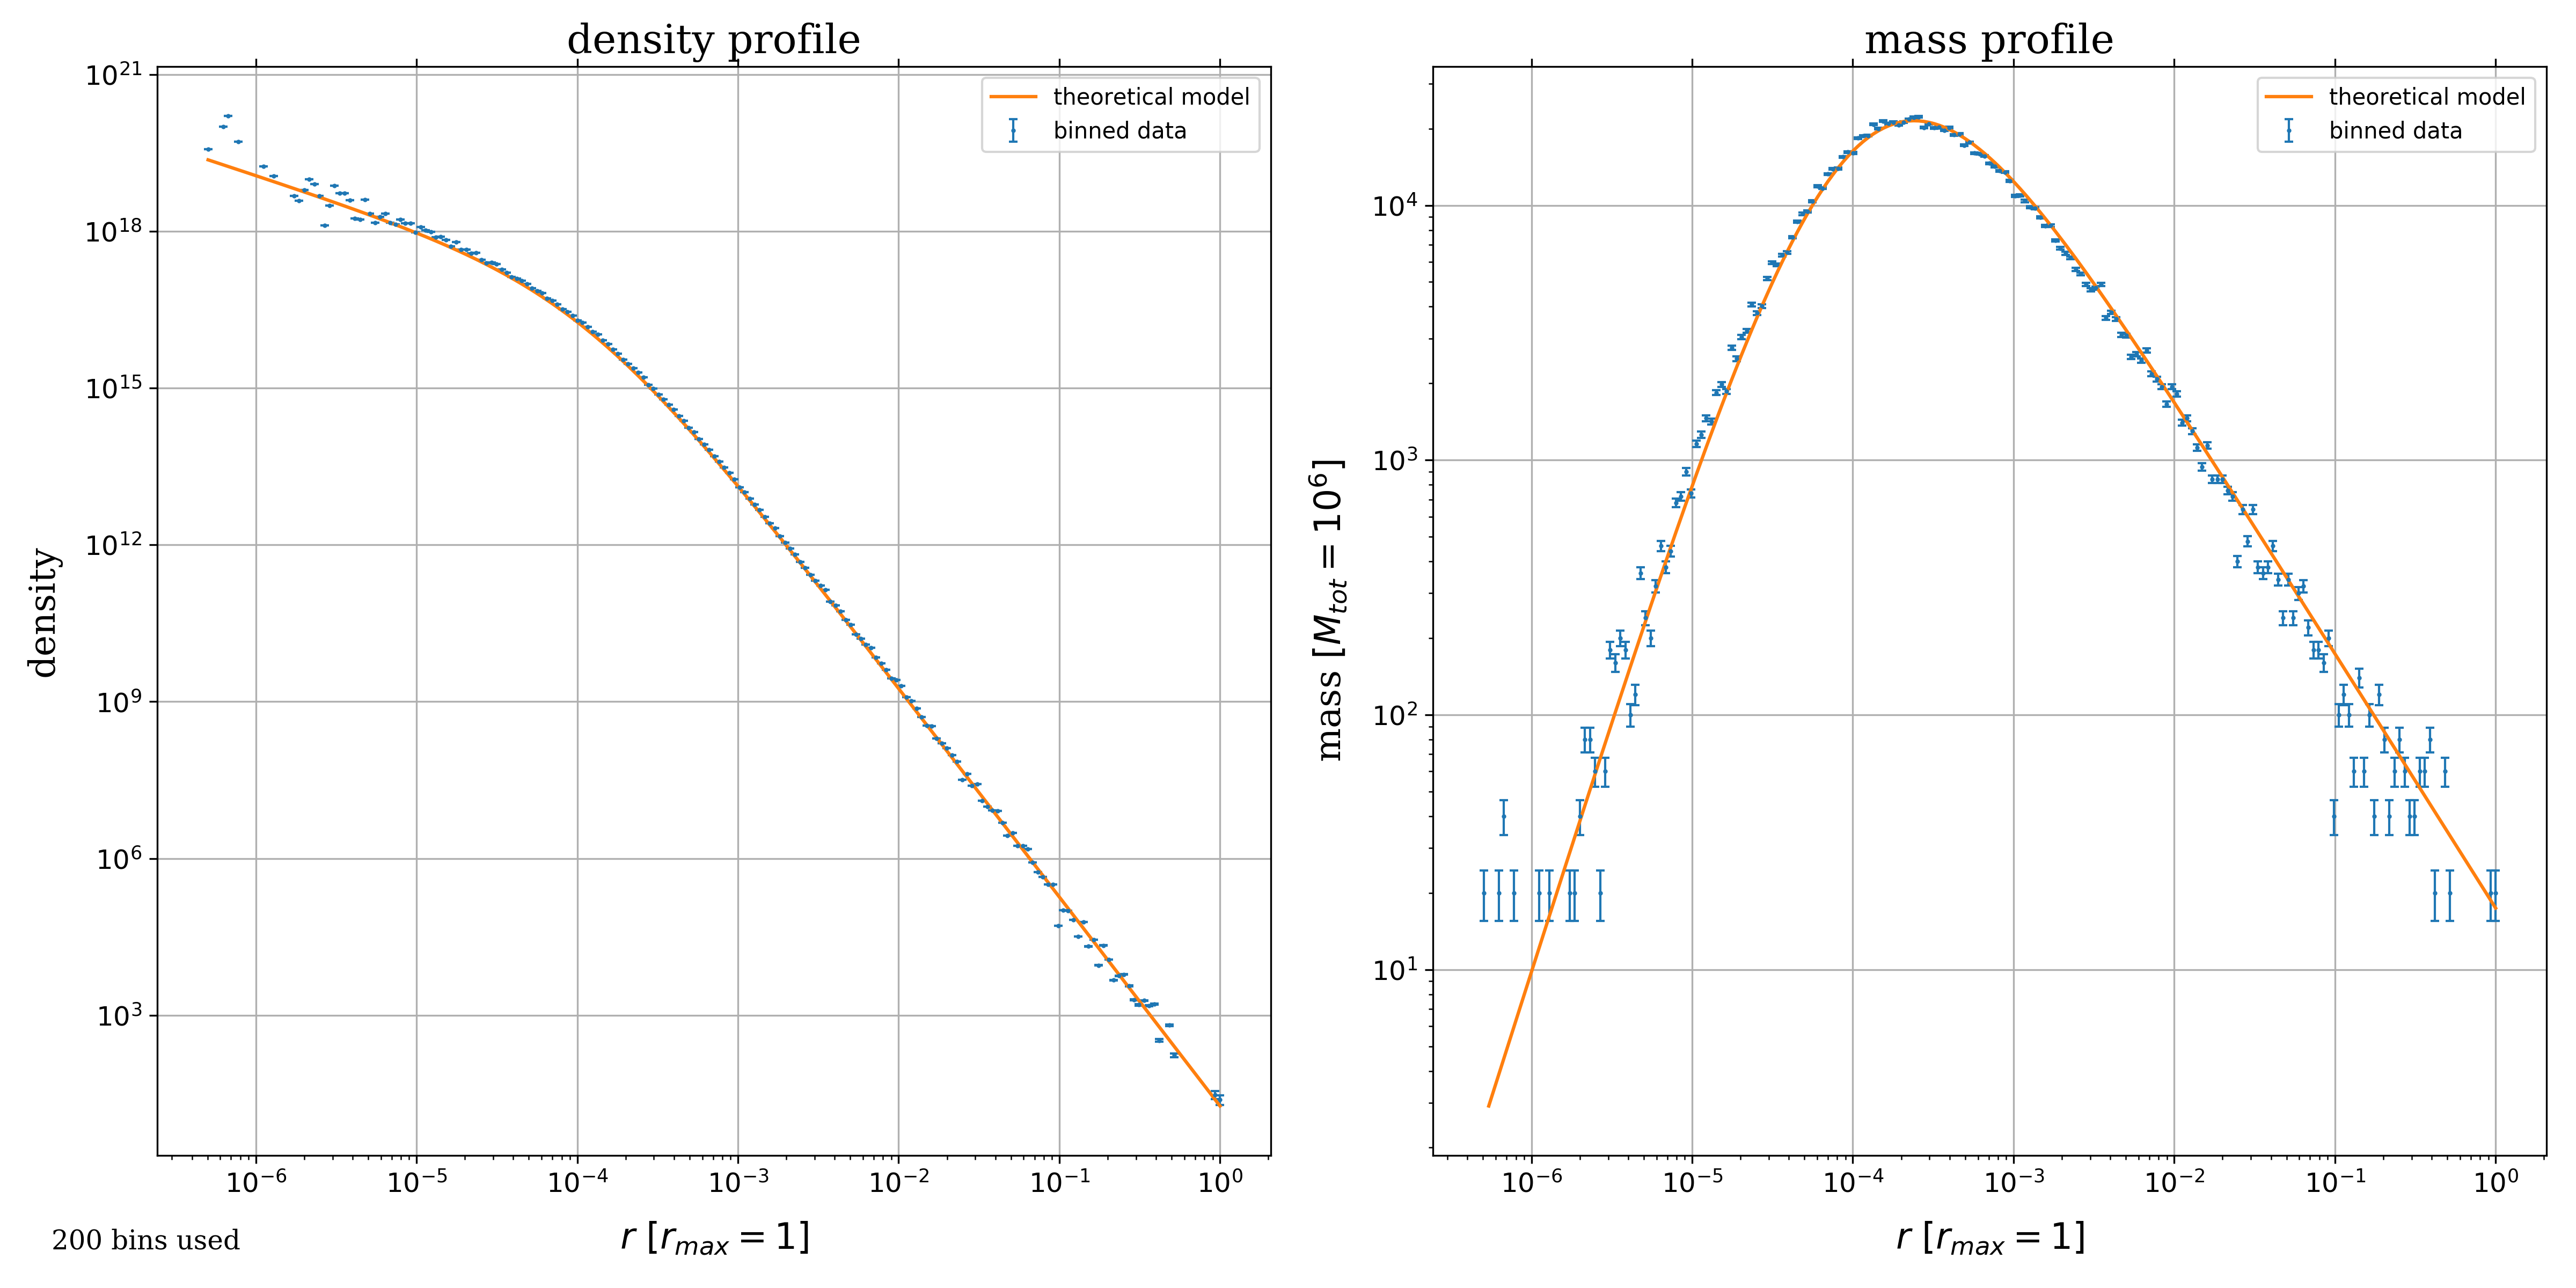
\includegraphics[width=\linewidth]{../results/density_plot/step0_density_plot.png}
	
	\alert{Only in this plot:} $M_{tot} \equiv 10^6$ so that the errorbars don't dominate the plot.
\end{frame}






\section{Direct Force Calculation}

\begin{frame}
	\frametitle{Direct forces calculation}
	
	Acceleration of particle $i$:
	\begin{align*}
		\ddot{\mathbf{r}}_i = - G \sum\limits_{j=1}^{N}  \frac{m_j}{[(\mathbf{r}_i - \mathbf{r}_j)^2 + \epsilon^2 ]^{\frac{3}{2}}} (\mathbf{r}_i - \mathbf{r}_j)
	\end{align*}

$\epsilon$ is the \textit{softening length}. It's purposes are:
\begin{itemize}
	\item computational efficiency
	\item avoid large angle scatterings
	\item avoid expense to calculate orbits in a singular potential
	\item prevent the possibility of formation of bound particle pairs
\end{itemize}
	
\end{frame}






\begin{frame}
	\frametitle{Direct force calculation results for varying softening}
	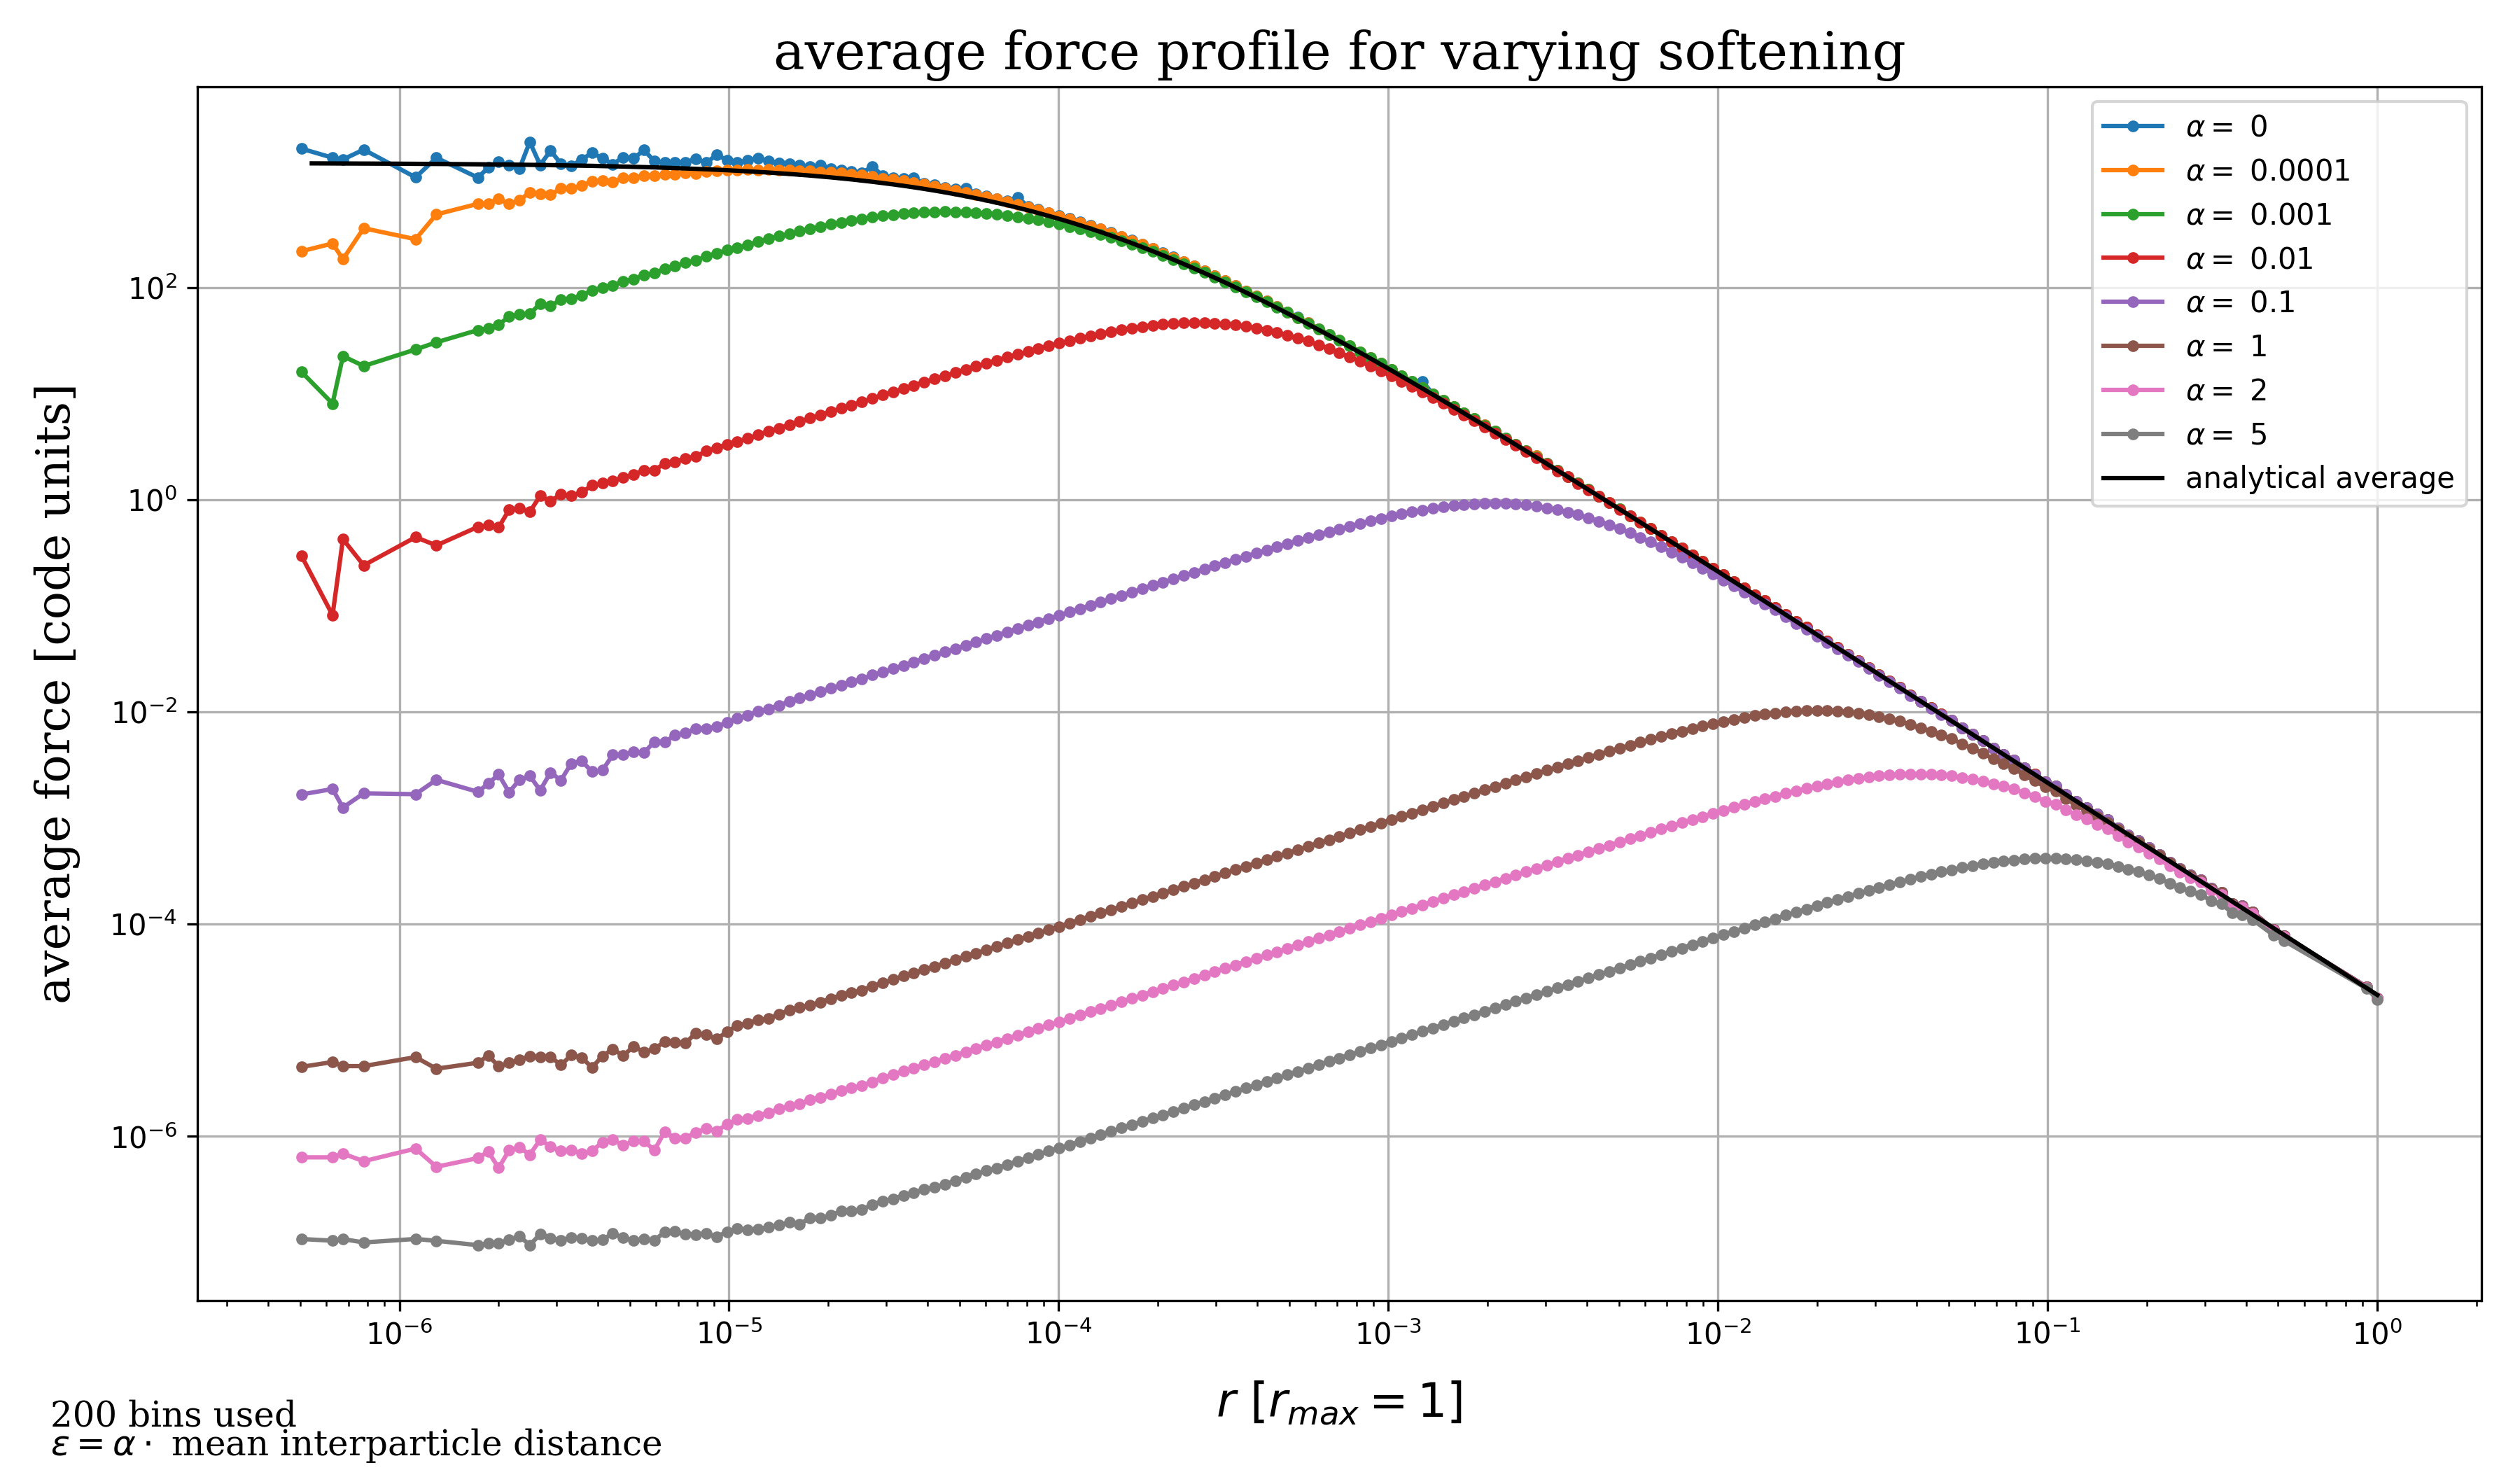
\includegraphics[width=\textwidth]{../results/average_direct_force/average_force_plot.png}
\end{frame}



\section{Hierarchical Multipole Method}

\begin{frame}
	\frametitle{Hierarchical Multipole Method}
	\begin{columns}
		\column{.7\textwidth}
			Central idea: use the multipole expansion of a distant group of particles to describe its gravity, instead of summing up the forces from all individual particles.			
			(For close groups, I use direct force calculation.)\\[1em]
			
			Multipole expansion of the potential gives:
			\begin{align*}
				\Phi(\mathbf{r}) &= -G \left( \frac{M}{|\mathbf{y}|} + \frac{1}{2} \frac{\mathbf{y}^T\mathbf{Q}\mathbf{y} }{\mathbf{|y|^5}} \right)\\
				\mathbf{y} &= \mathbf{r} - \mathbf{s}\\
				Q_{ij} &= \sum_k m_k [3(\mathbf{s} - \mathbf{x_k})_i(\mathbf{s} - \mathbf{x_k})_j - \delta_{ij} (\mathbf{s} - \mathbf{x_k})^2]
			\end{align*}
			
		\column{.3\textwidth}
			\centering
			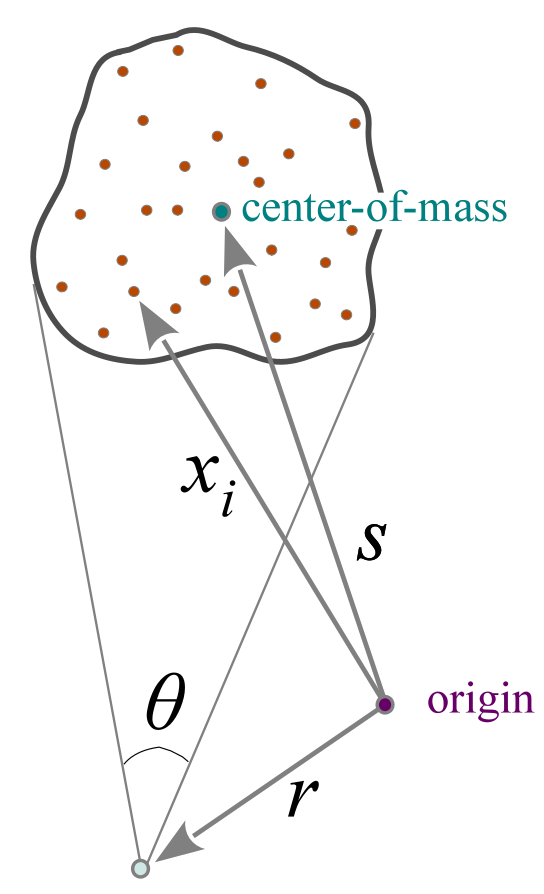
\includegraphics[width=\textwidth]{images/multipole.png} 
	\end{columns}

	The expansion is valid for $\theta \approx \frac{l}{y} \ll 1$
\end{frame}





\begin{frame}
	The particles are grouped hierarchically and the multipole moments are pre-computed for later use.
	
	I used the Barnes-Hut oct-tree: Assume particles are in a cube. The cube is then recursively subdivided into 8 sub-cubes of half the size in each spatial dimension, until each sub-cube contains only a single particle (or some other user-set limit).\\[1em]
	
	\textbf{Force calculation}: 
	
	For all leaf cells:
	
	\quad For all root cells:
	
	\quad\quad walk tree (this leaf cell, root cell)
	
	
	
\end{frame}




\begin{frame}
	\textbf{Walking the tree} (target cell, source cell):
	

	If source cell is leaf cell: Use direct force calculation, end walk for this source.
	
	If target (leaf) cell is inside this source cell:
	
	\quad for all children of the source cell:
	
	\quad \quad walk the tree (target, child of source)


	If target (leaf) cell is \textit{not} inside this source cell:
	
	\quad if $\theta < \theta_{max}$: Calculate multipole force, stop walk for this source
	
	\quad else: for all children of the source cell:
	
	\quad \quad walk the tree (target, child of source)
\end{frame}







\begin{frame}
	\begin{columns}
		\column{.33\textwidth}
			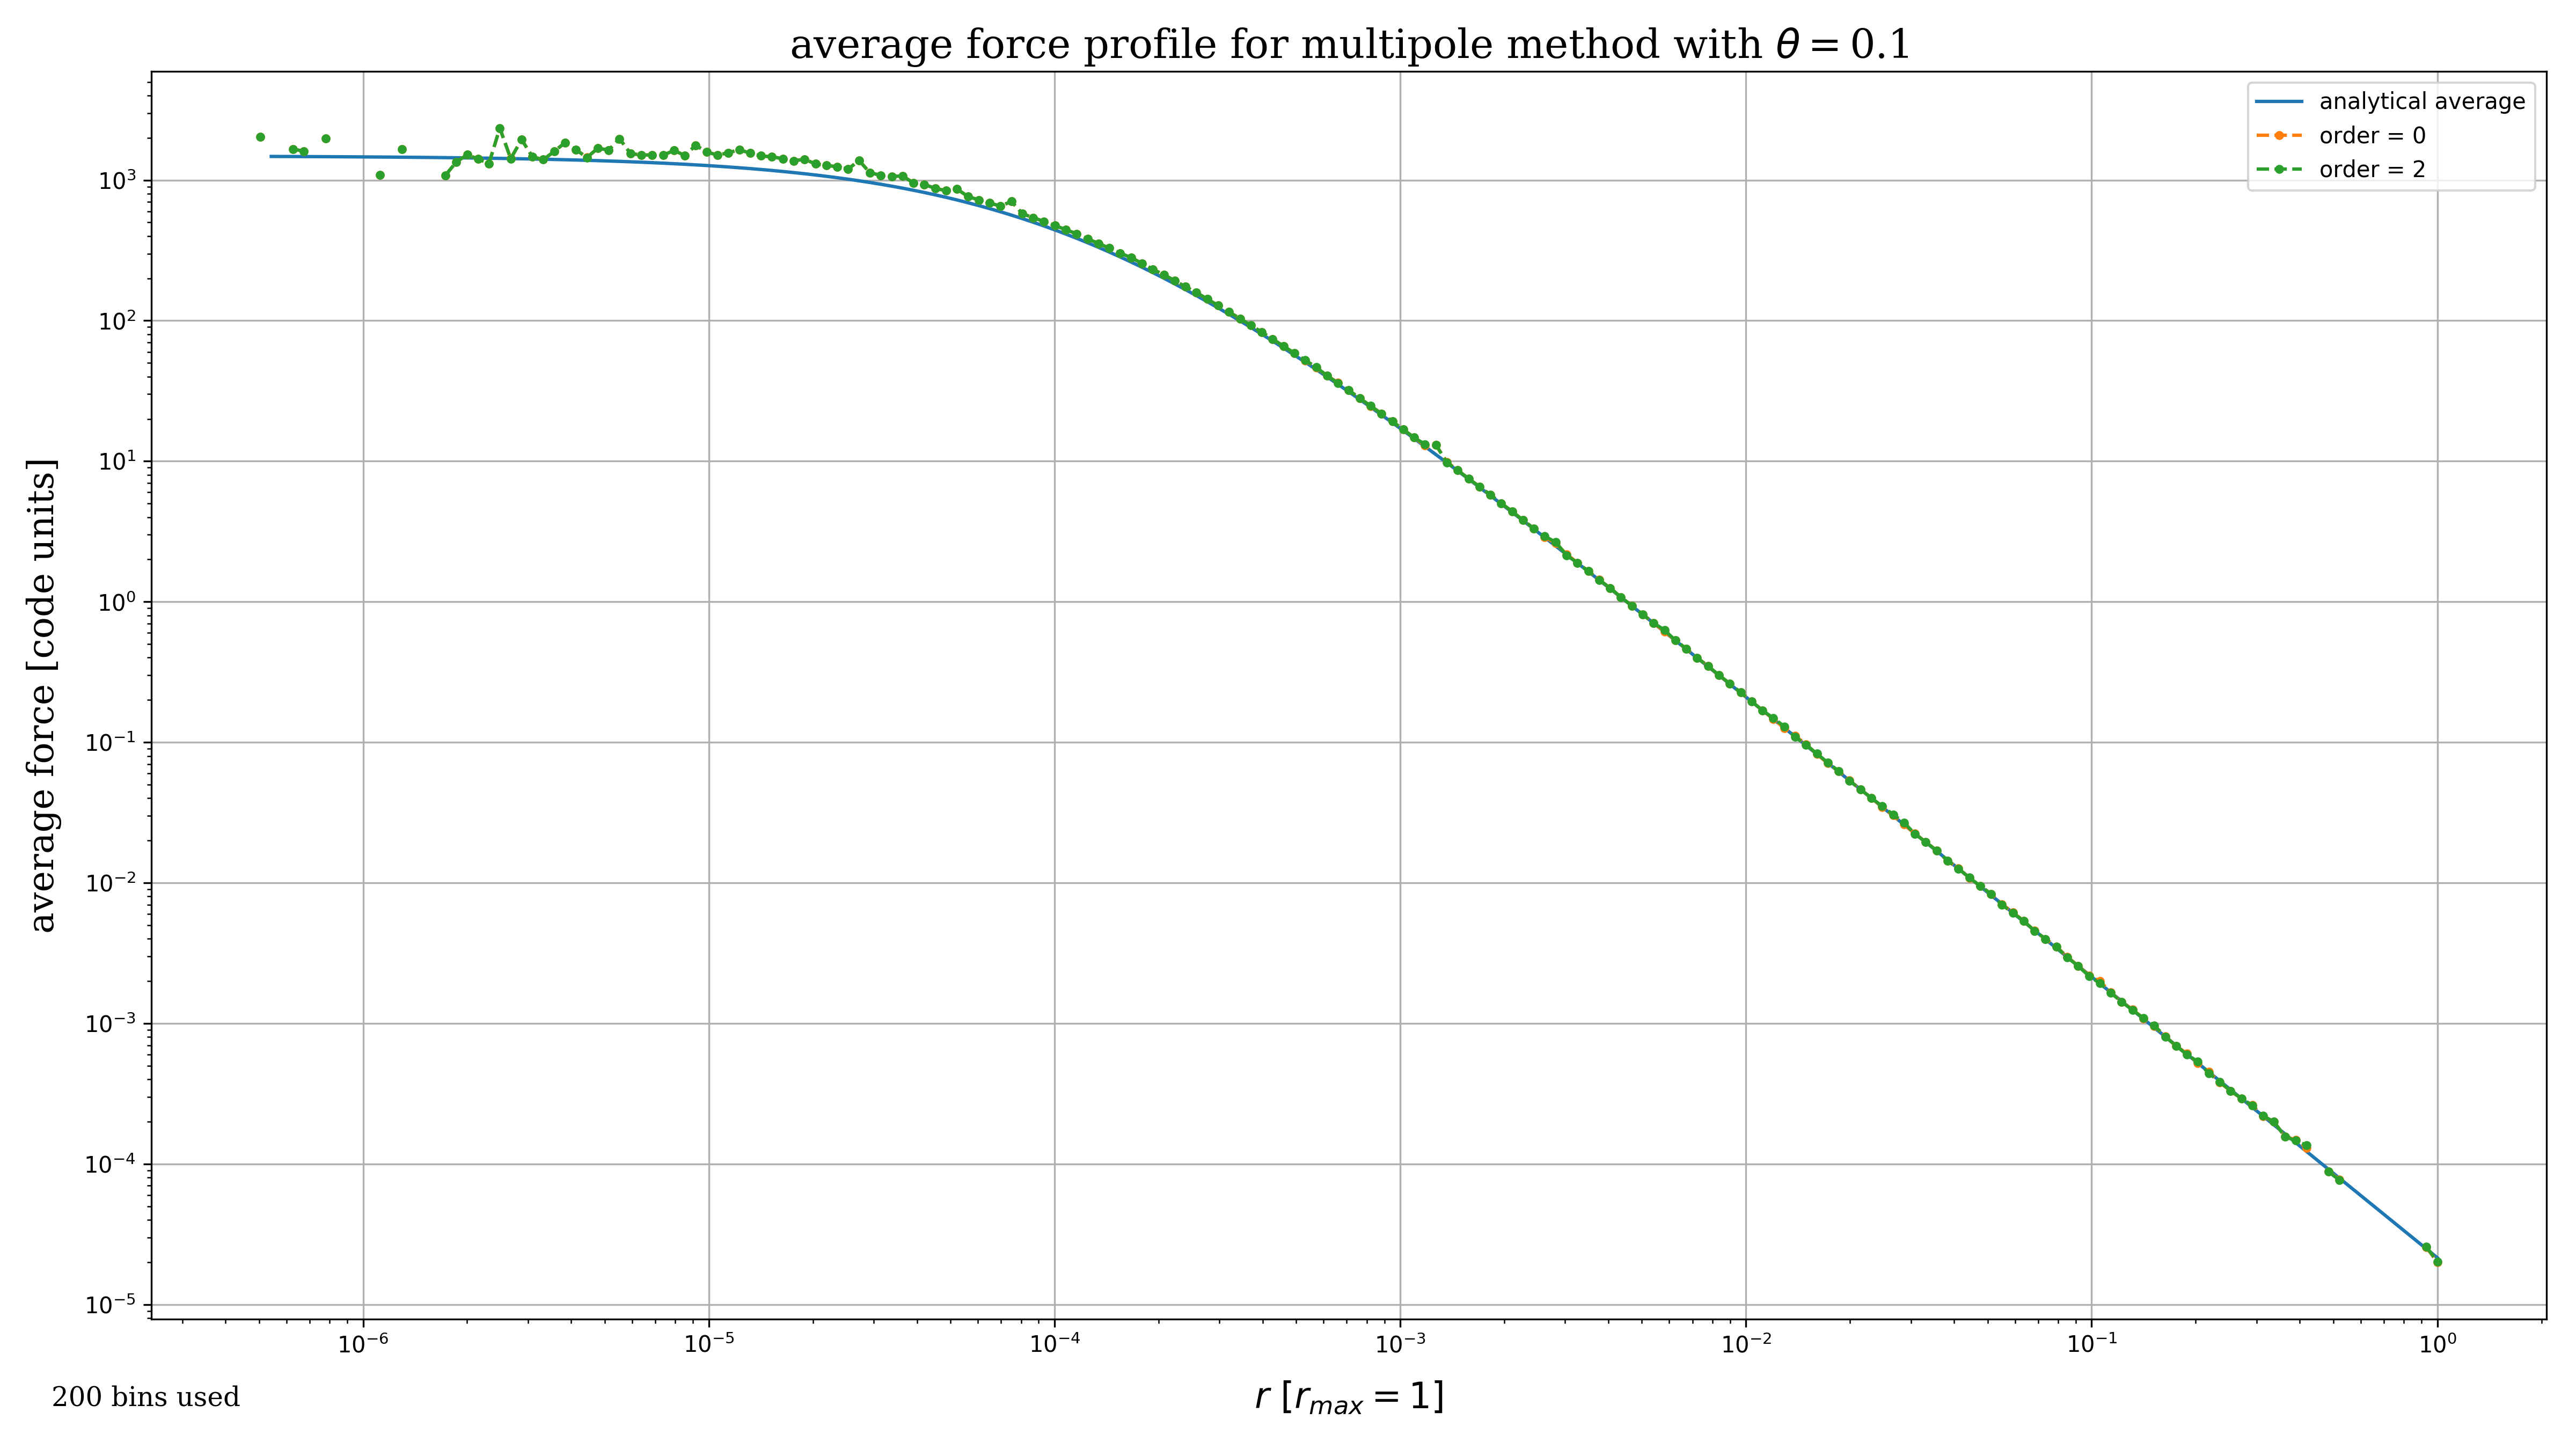
\includegraphics[width=\textwidth]{../results/multipole_forces/bucket01/0.1/multipole_forces_plot-0.1.png}\\[2em]
			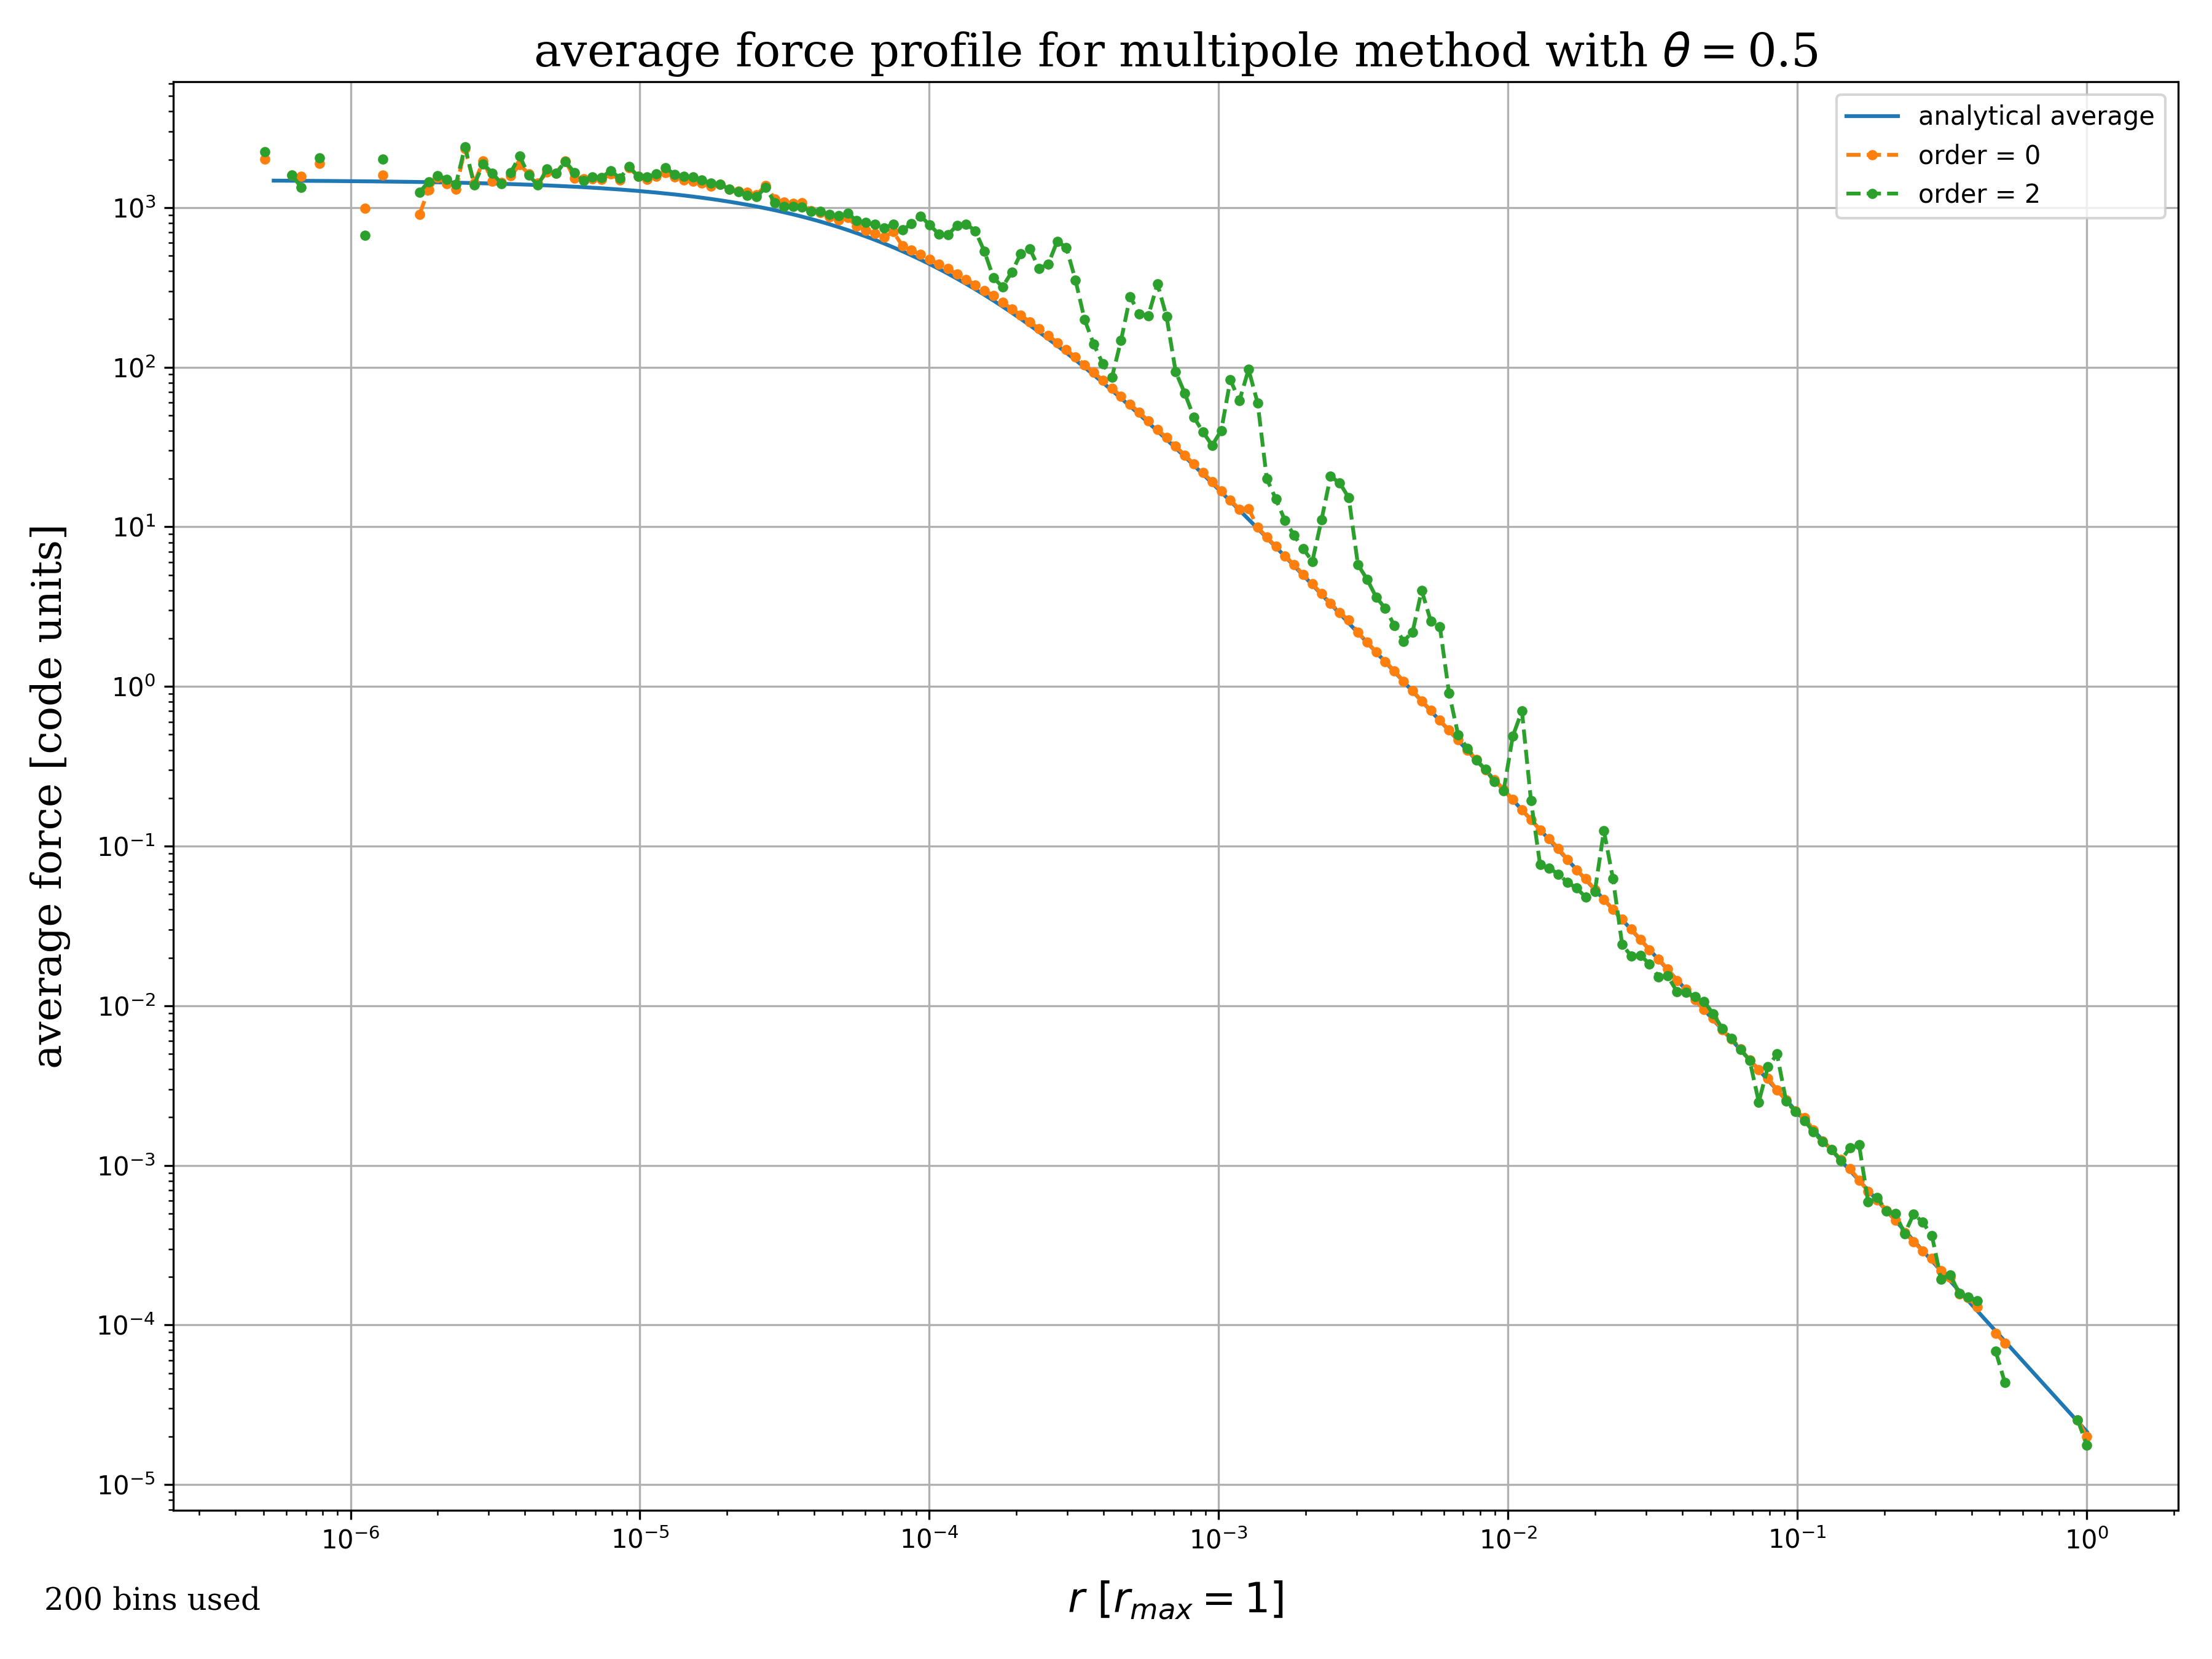
\includegraphics[width=\textwidth]{../results/multipole_forces/bucket01/0.5/multipole_forces_plot-0.5.png}
		\column{.33\textwidth}
			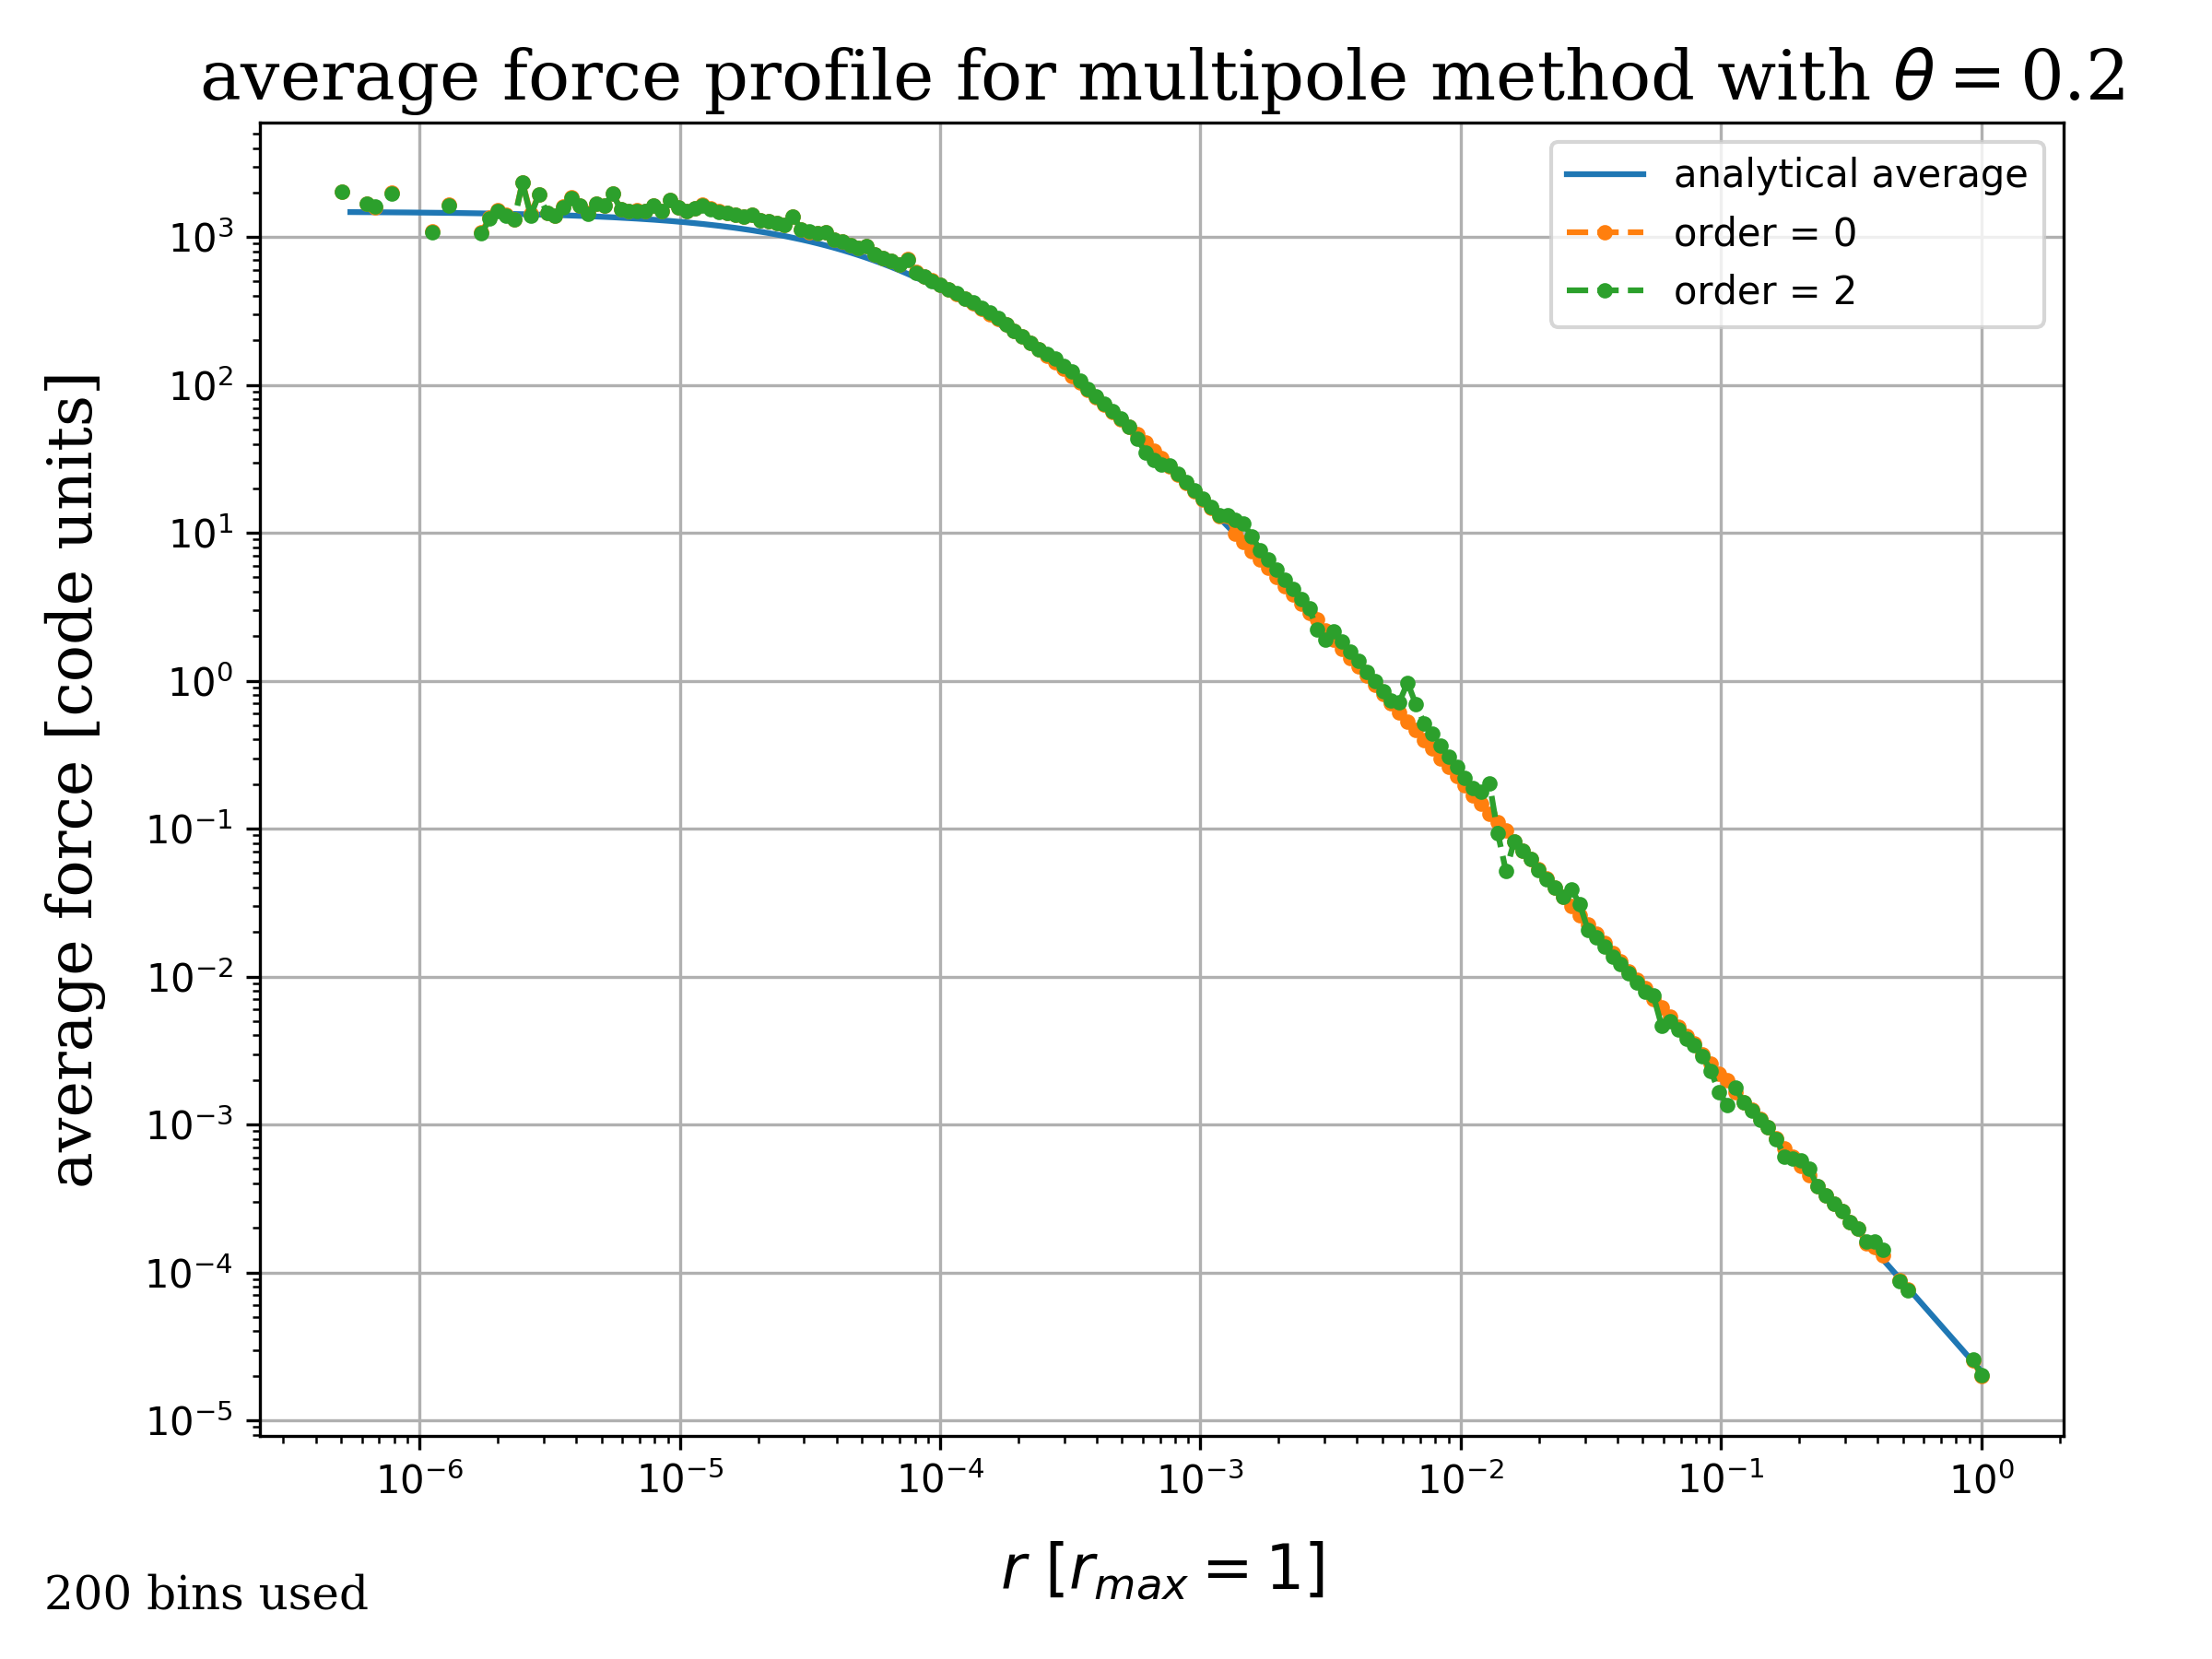
\includegraphics[width=\textwidth]{../results/multipole_forces/bucket01/0.2/multipole_forces_plot-0.2.png}\\[2em]
			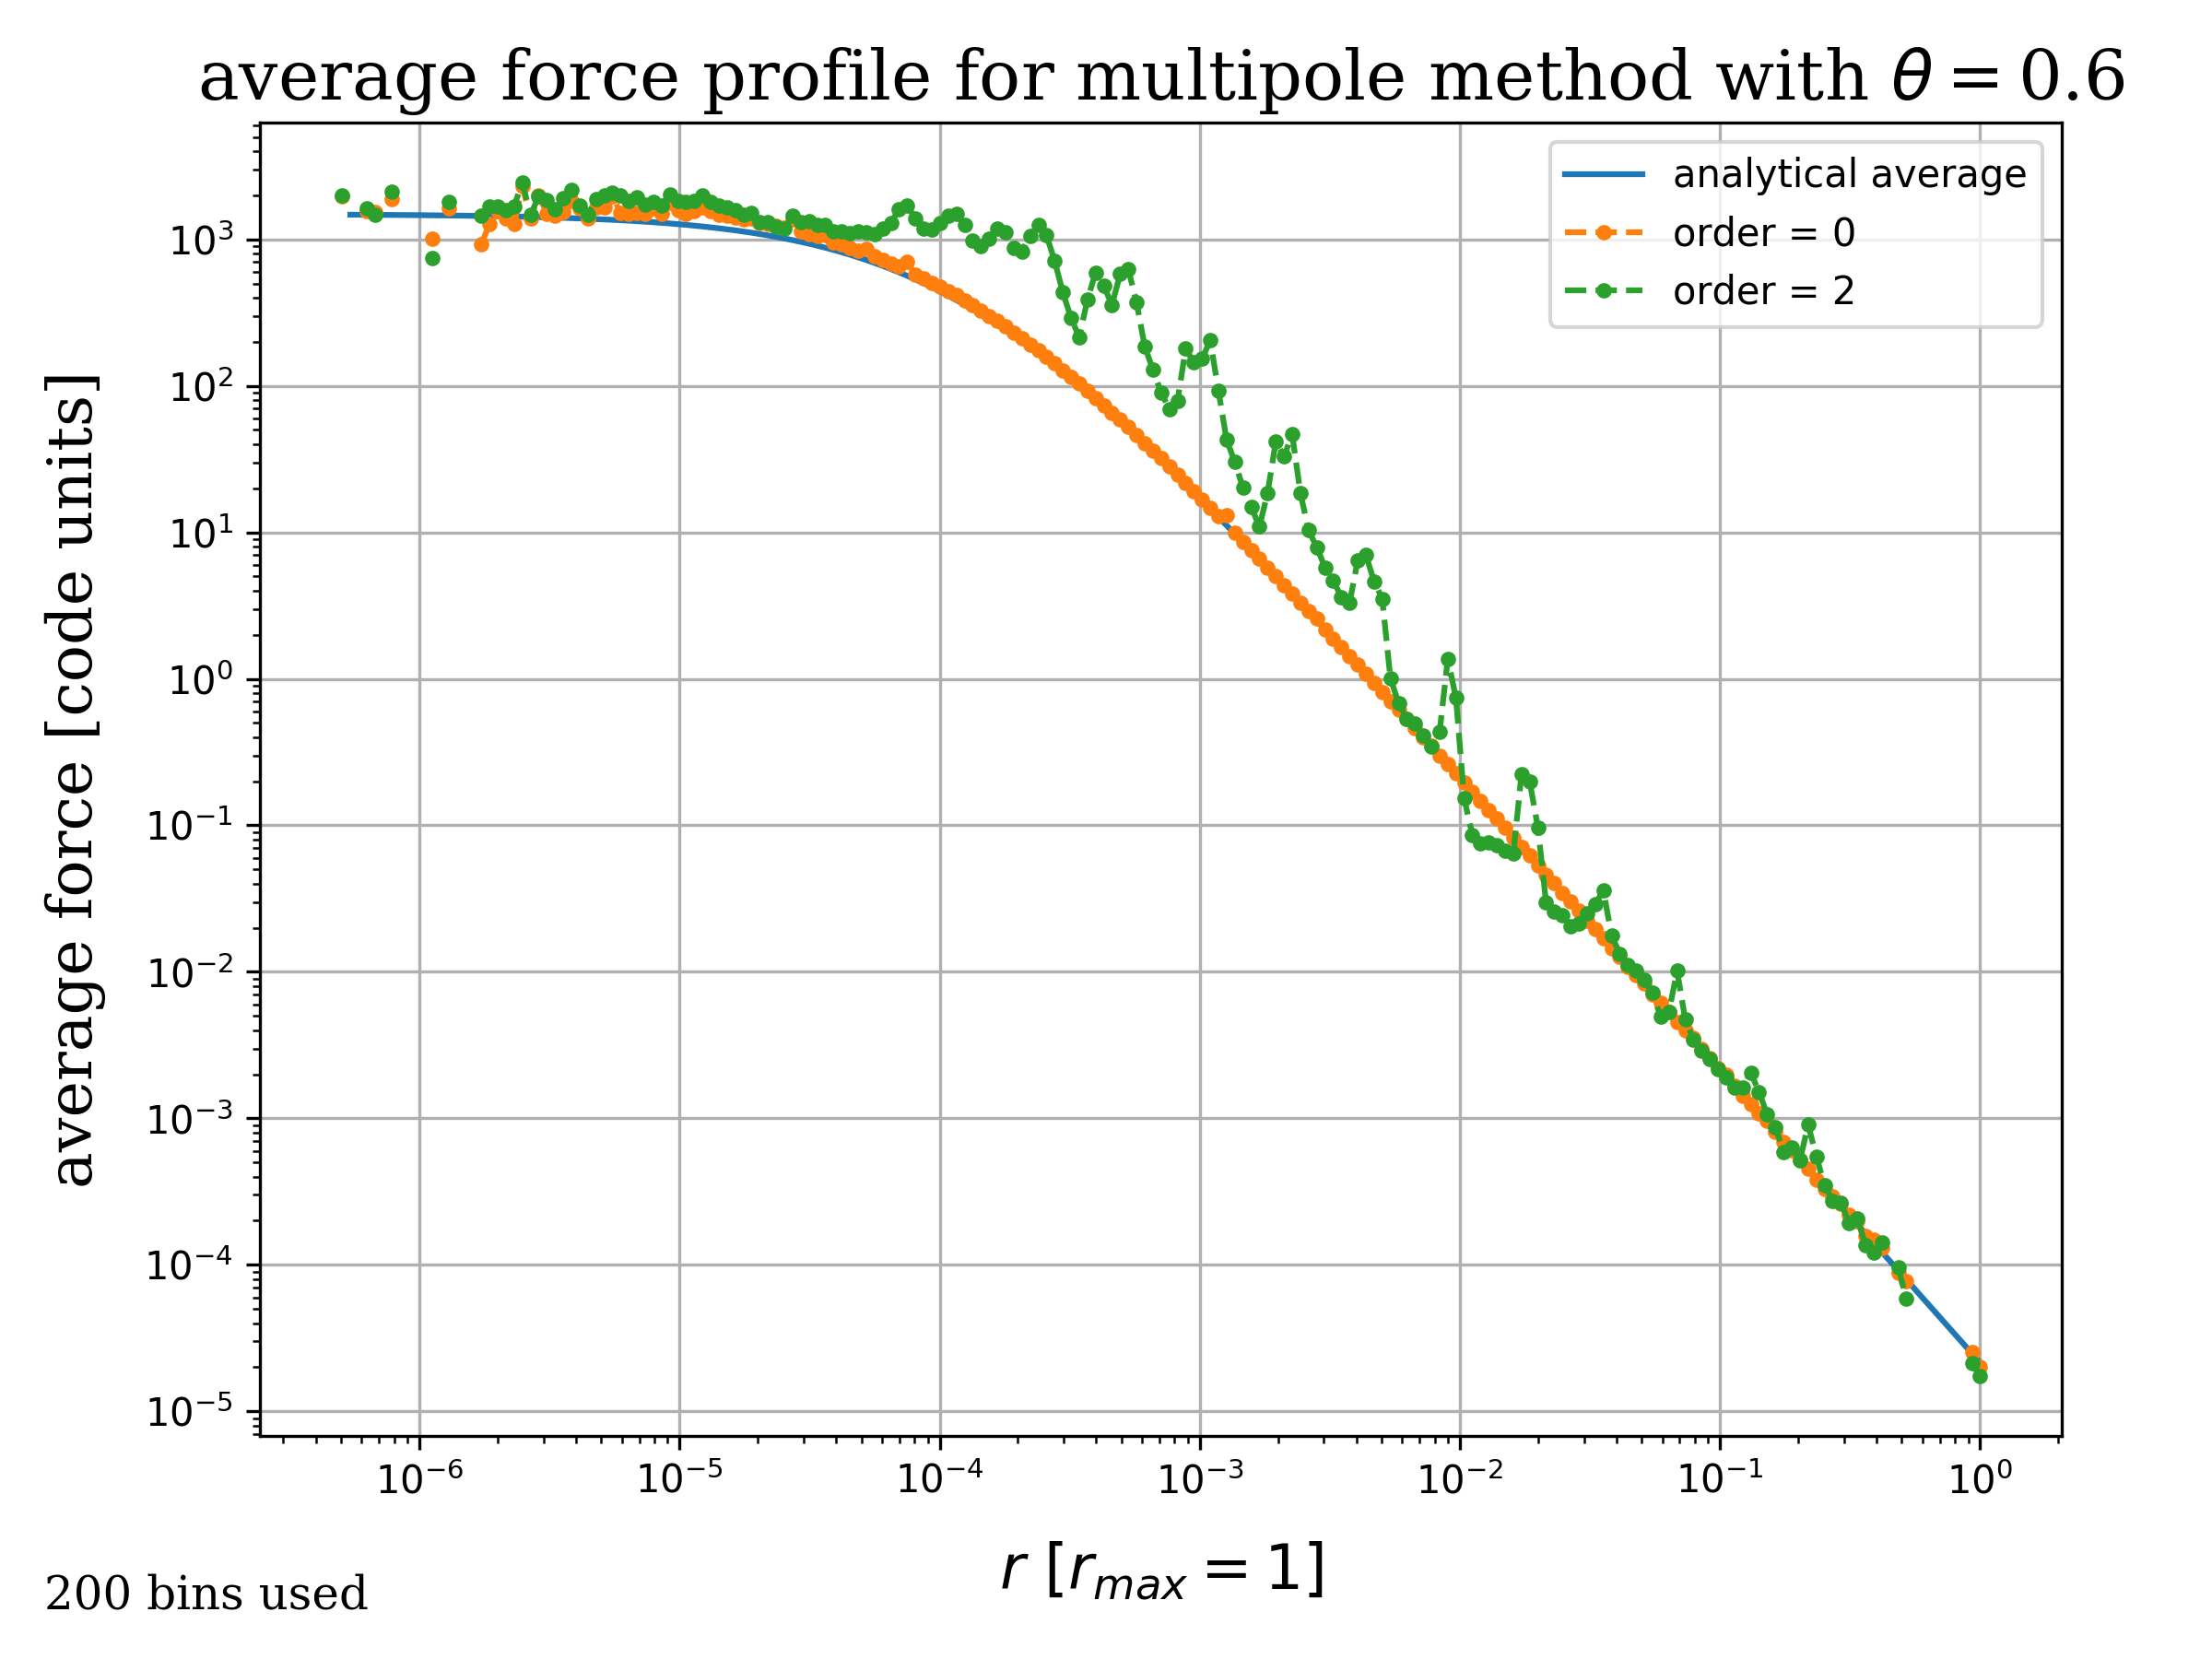
\includegraphics[width=\textwidth]{../results/multipole_forces/bucket01/0.6/multipole_forces_plot-0.6.png}
		\column{.33\textwidth}
			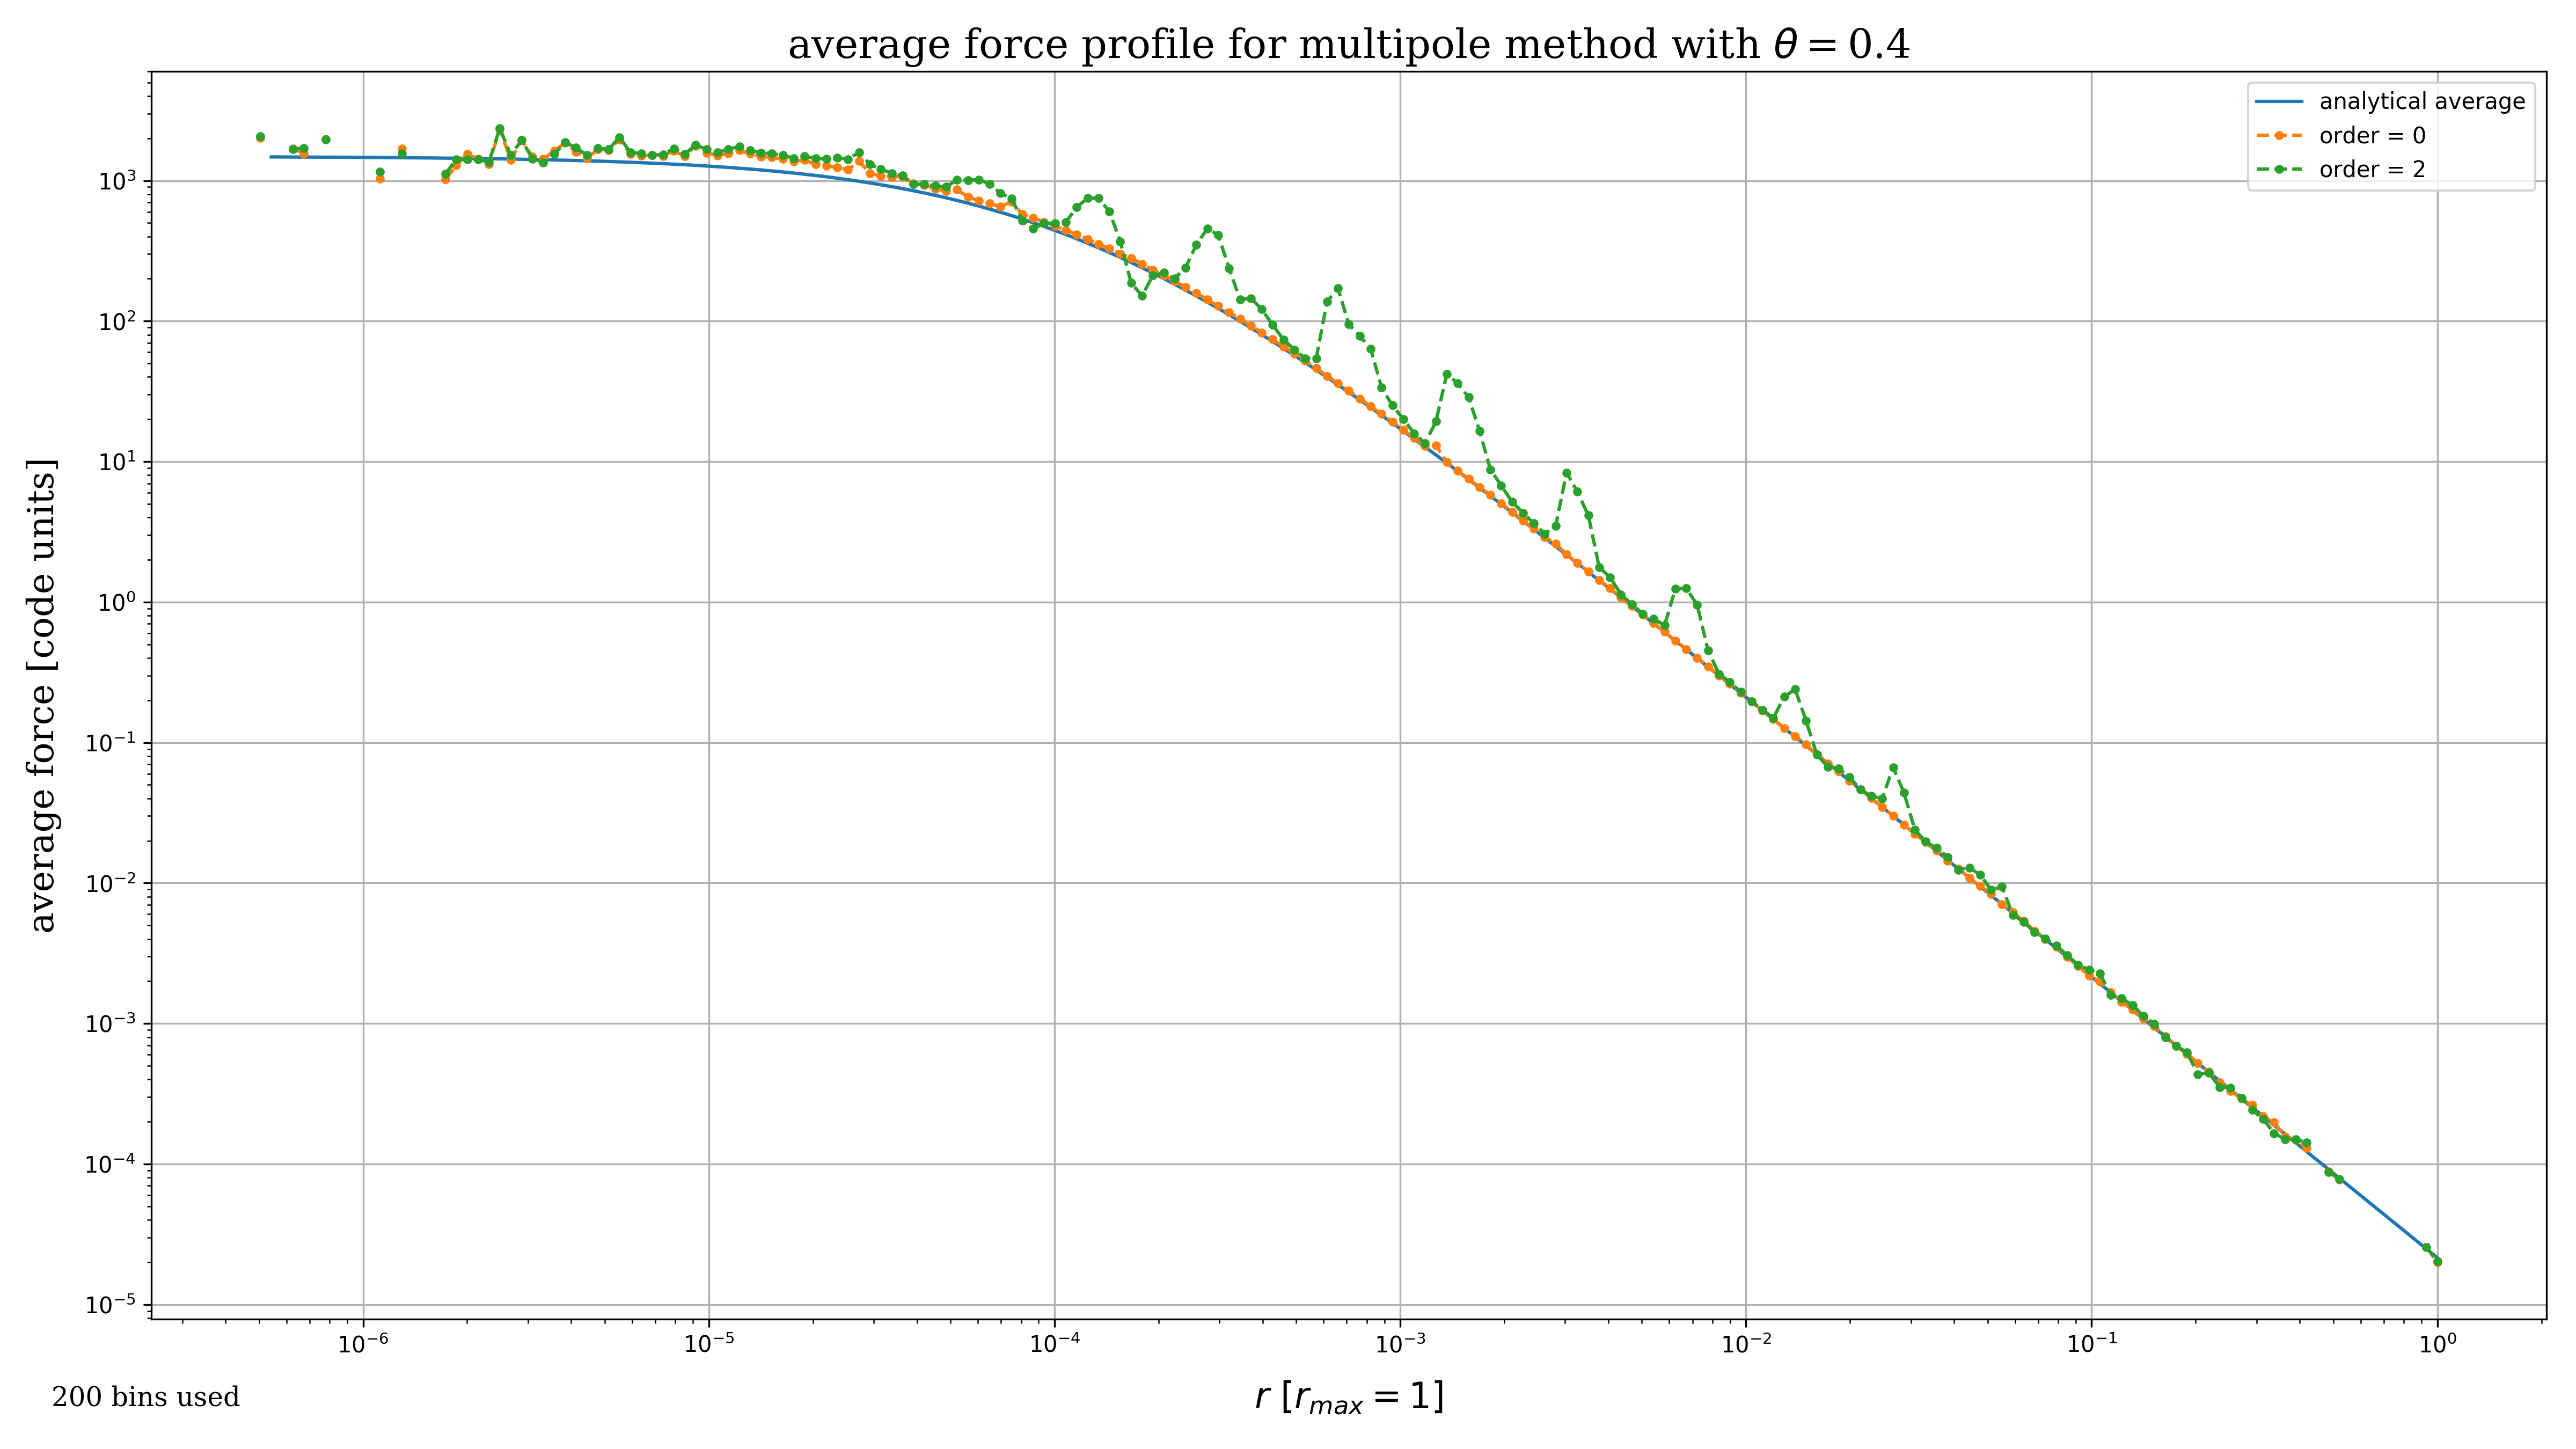
\includegraphics[width=\textwidth]{../results/multipole_forces/bucket01/0.4/multipole_forces_plot-0.4.png}\\[2em]
			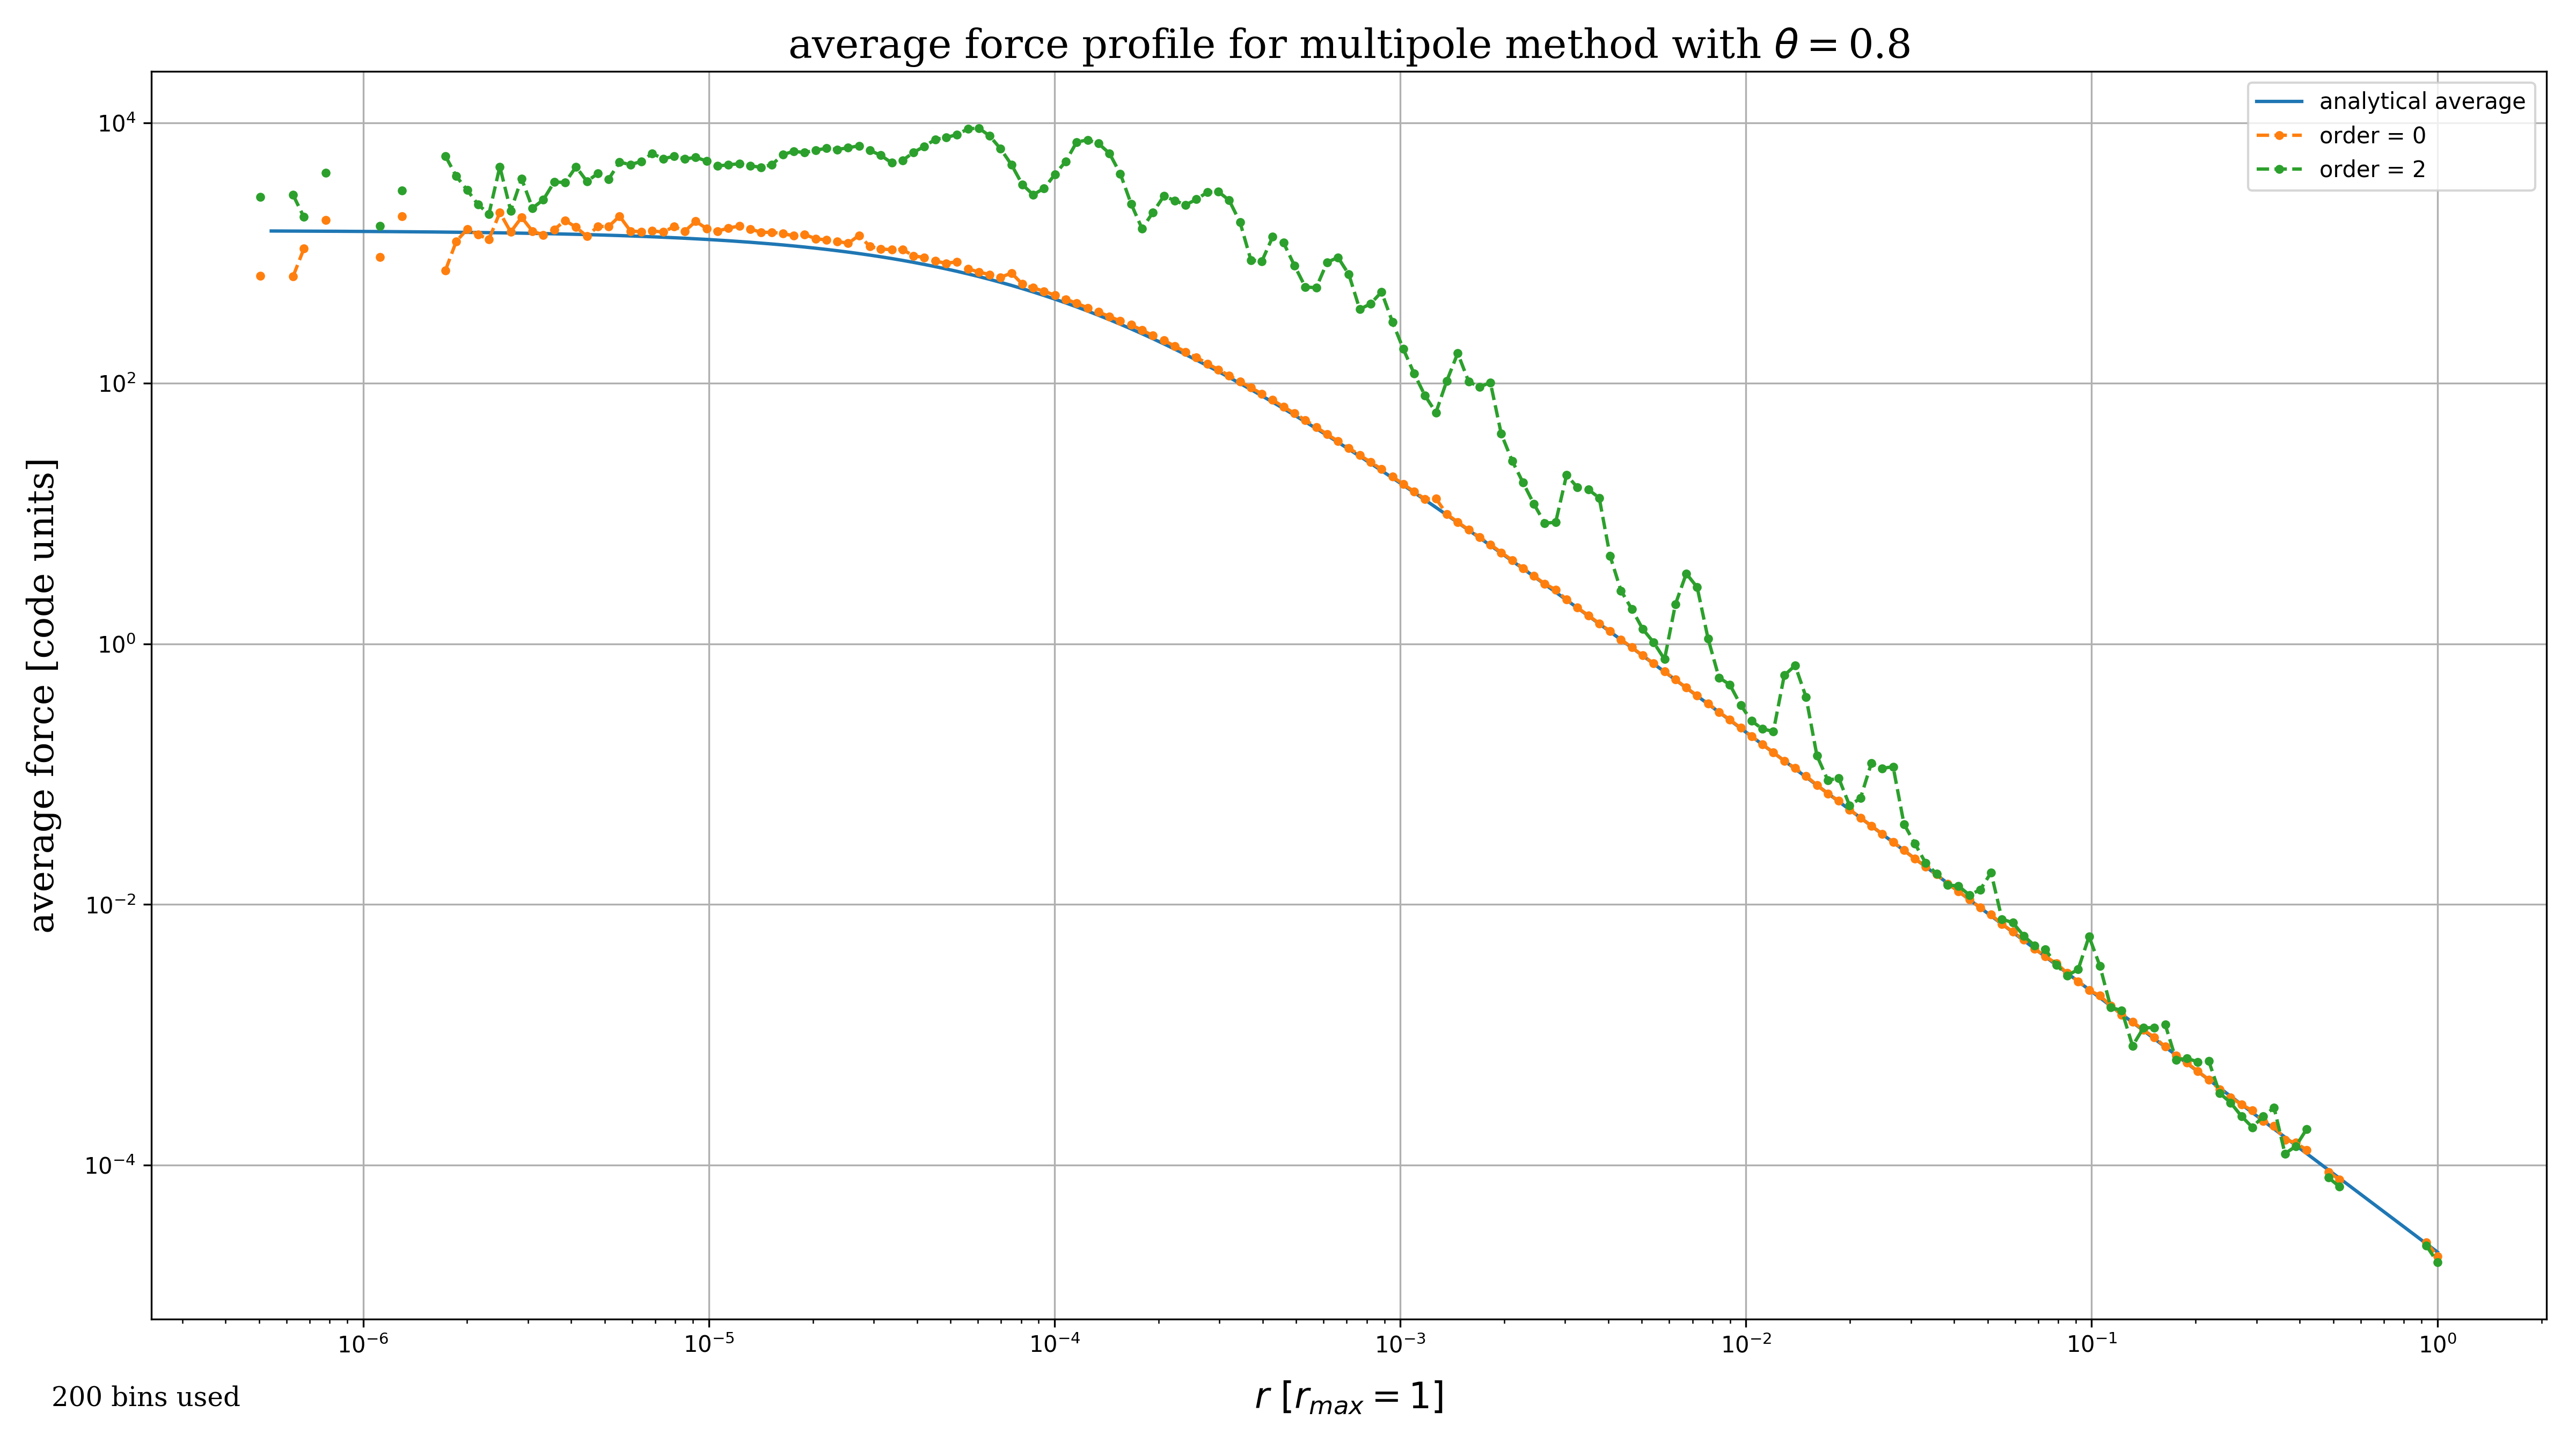
\includegraphics[width=\textwidth]{../results/multipole_forces/bucket01/0.8/multipole_forces_plot-0.8.png}
	\end{columns}
\end{frame}





\begin{frame}
	\frametitle{Comparison Direct vs multipole calculation}
	
	Estimating accuracy with the $L1$ norm: $L1 = \frac{1}{N} \sum\limits_i |\bar{F}_i - \bar{F}_{analytical}(r_i)|$, where $\bar{F}_{analytical}(r_i)$  is the analytical average force at $r_i$.
	
	For both the direct forces and multipole method, $\epsilon = 0.01 \cdot mid$. Shown are the relative values for both monopole and quadrupole oders, relative to the values for the direct forces calculation.
	
	\centering
	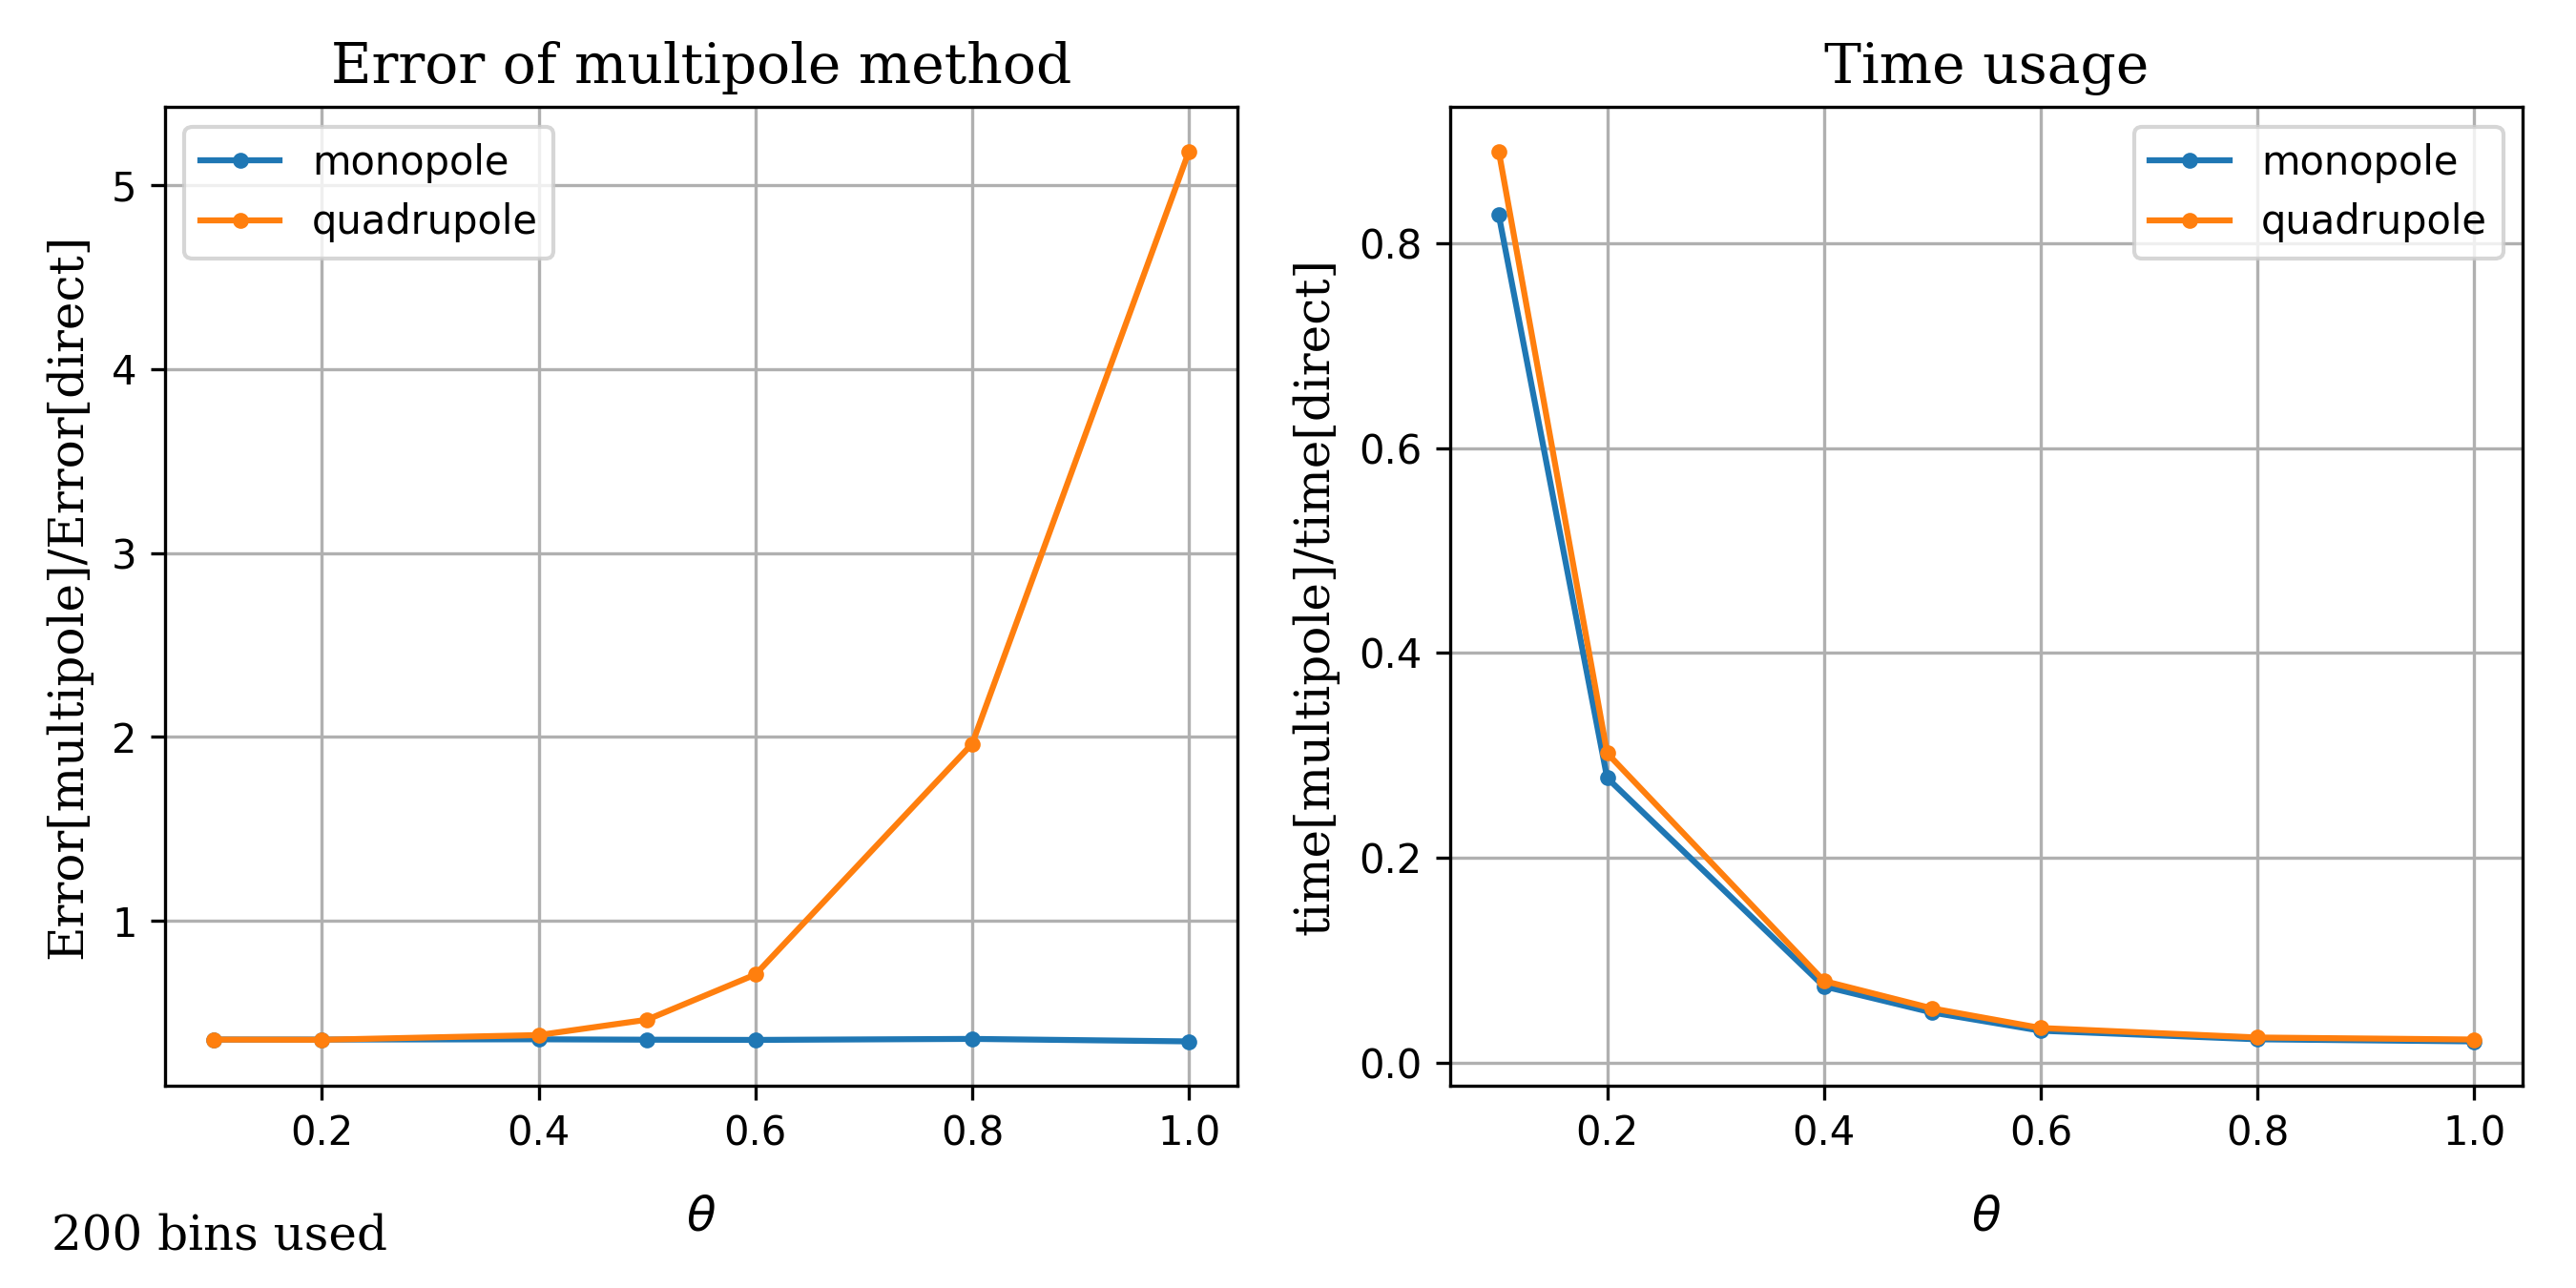
\includegraphics[width=\textwidth]{../results/multipole_forces/compare_direct_multipole.png}
\end{frame}






\begin{frame}[fragile]
	Program, plotting scripts and this presentation available on \verb!https://bitbucket.org/mivkov/computational_astrophysics!
\end{frame}








\end{document}
